
\newpage
\section{پیاده سازی ساز و کار سیناپس}
    در این بخش، میخواهیم ساز و کار سیناپس را با استفاده از تابع دلتای دیراک
    \footnote{\lr{Delta Dirac function}}
    پیاده سازی کنیم. جزئیات پیاده سازی در فایل های کد آماده است و فقط در اینجا به نحوه پیاده سازی و همچنین آزمایش آن با یک و دو جمعیت نورونی می پردازیم.

    طبق لینک داده شده، در تجزیه و تحلیل ریاضی، تابع دلتای دیراک
    (یا توزیع $\delta$)، 
    همچنین به عنوان تکانه واحد شناخته می شود، یک تابع تعمیم یافته بر روی اعداد واقعی است که مقدار آن در همه جا صفر است به جز صفر، و انتگرال آن در کل محور حقیقی. برابر یک است.
    \footnote{\href{https://en.wikipedia.org/wiki/Dirac\_delta\_function}{ویکی پدیا}}

    از این رو برای پیاده سازی آن به این صورت عمل میکنیم که ابتدا یک ماتریس به نام 
    $W$ 
    به ابعاد تعداد نورون های پیش سیناپسی
    ($m$)
    در تعداد نورون های پس سیناپسی
    ($n$) 
    ایجاد میکنیم که ماتریس 
    \textbf{وزن}
    های سیناپس ما را تشکیل می دهد.
    ($W_{m\times n}$)
    در هر تکرار
    \footnote{iteration}
    از شبیه سازی، اندیس نورون های پیش سیناپسی که در تکرار قبلی ضربه 
    \footnote{spike}
    زده اند را در یک متغیر مانند 
    \texttt{pre\_spike}
    ذخیره کرده، و از ماتریس وزن ها
    ($W$)
    سطر هایی که ضربه زده اند را جدا کرده و سپس برای هر یک از نورون های پیش سیناپسی و اندیس متناظر، مجموع این وزن ها را حساب کرده و به عنوان جریان سیناپسی ورودی آن نورون در نظر میگیریم و در متغیری مانند 
    \texttt{sg.I}
    ذخیره میکنیم. حال باید این جریان را به جریان نورون های پس سیناپسی اضافه کنیم، اینکار میتواند به راحتی توسط یک رفتار
    \footnote{Behavior}
    به نام دندرایت پیاده سازی شود که در هر تکرار، جریان سیناپسی را به علاوه جریان ورودی نورون می کند:
    \begin{equation}
        I_{ng}(t) = I_{sg}(t-1) + I_{sg}(t)
    \end{equation}

    حال به بررسی رفتار یک یا دو جمعیت نورونی، با پارامتر های مختلف می پردازیم. در این قسمت فقط الگوی ارتباط کامل را بررسی میکنیم و بررسی دقیق تر ۳ الگو را به بخش دوم پروژه واگذار میکنیم.
    \subsection{بررسی رفتار درون یک جمعیت نورونی}
        \subsubsection*{جمعیت نورونی بدون سیناپس}
        برای درک بهتر ساز و کار سیناپس ها، بهتر است ابتدا تاثیر آن را درون یک جمعیت نورونی به تنهایی بررسی کنیم. از این رو اول رفتار یک جمعیت را بدون حضور سیناپس و سپس در حضور سیناپس، بعد گذشت چند تکرار مشاهده میکنیم. 
        همانطور که در شکل 
        \ref{fig:part1-simple-ng}
        مشاهده می کنید، هنگامی که یک جریان ثابت به یک گروه نورونی یکسان وارد می شود، زمان ضربه زدن تمامی نورون ها در یک لحظه اتفاق میوفتد. دلیل این رفتار بدیهی است و بخاطر این است که از آنجا که نورون ها مقادیر یکسانی در هنگام شروع دارند و همچنین جریان یکسانی دریافت می کنند، زمان ضربه زدن آن ها نیز مشابه خواهد بود.
        \begin{figure}[!ht]
            \centering
            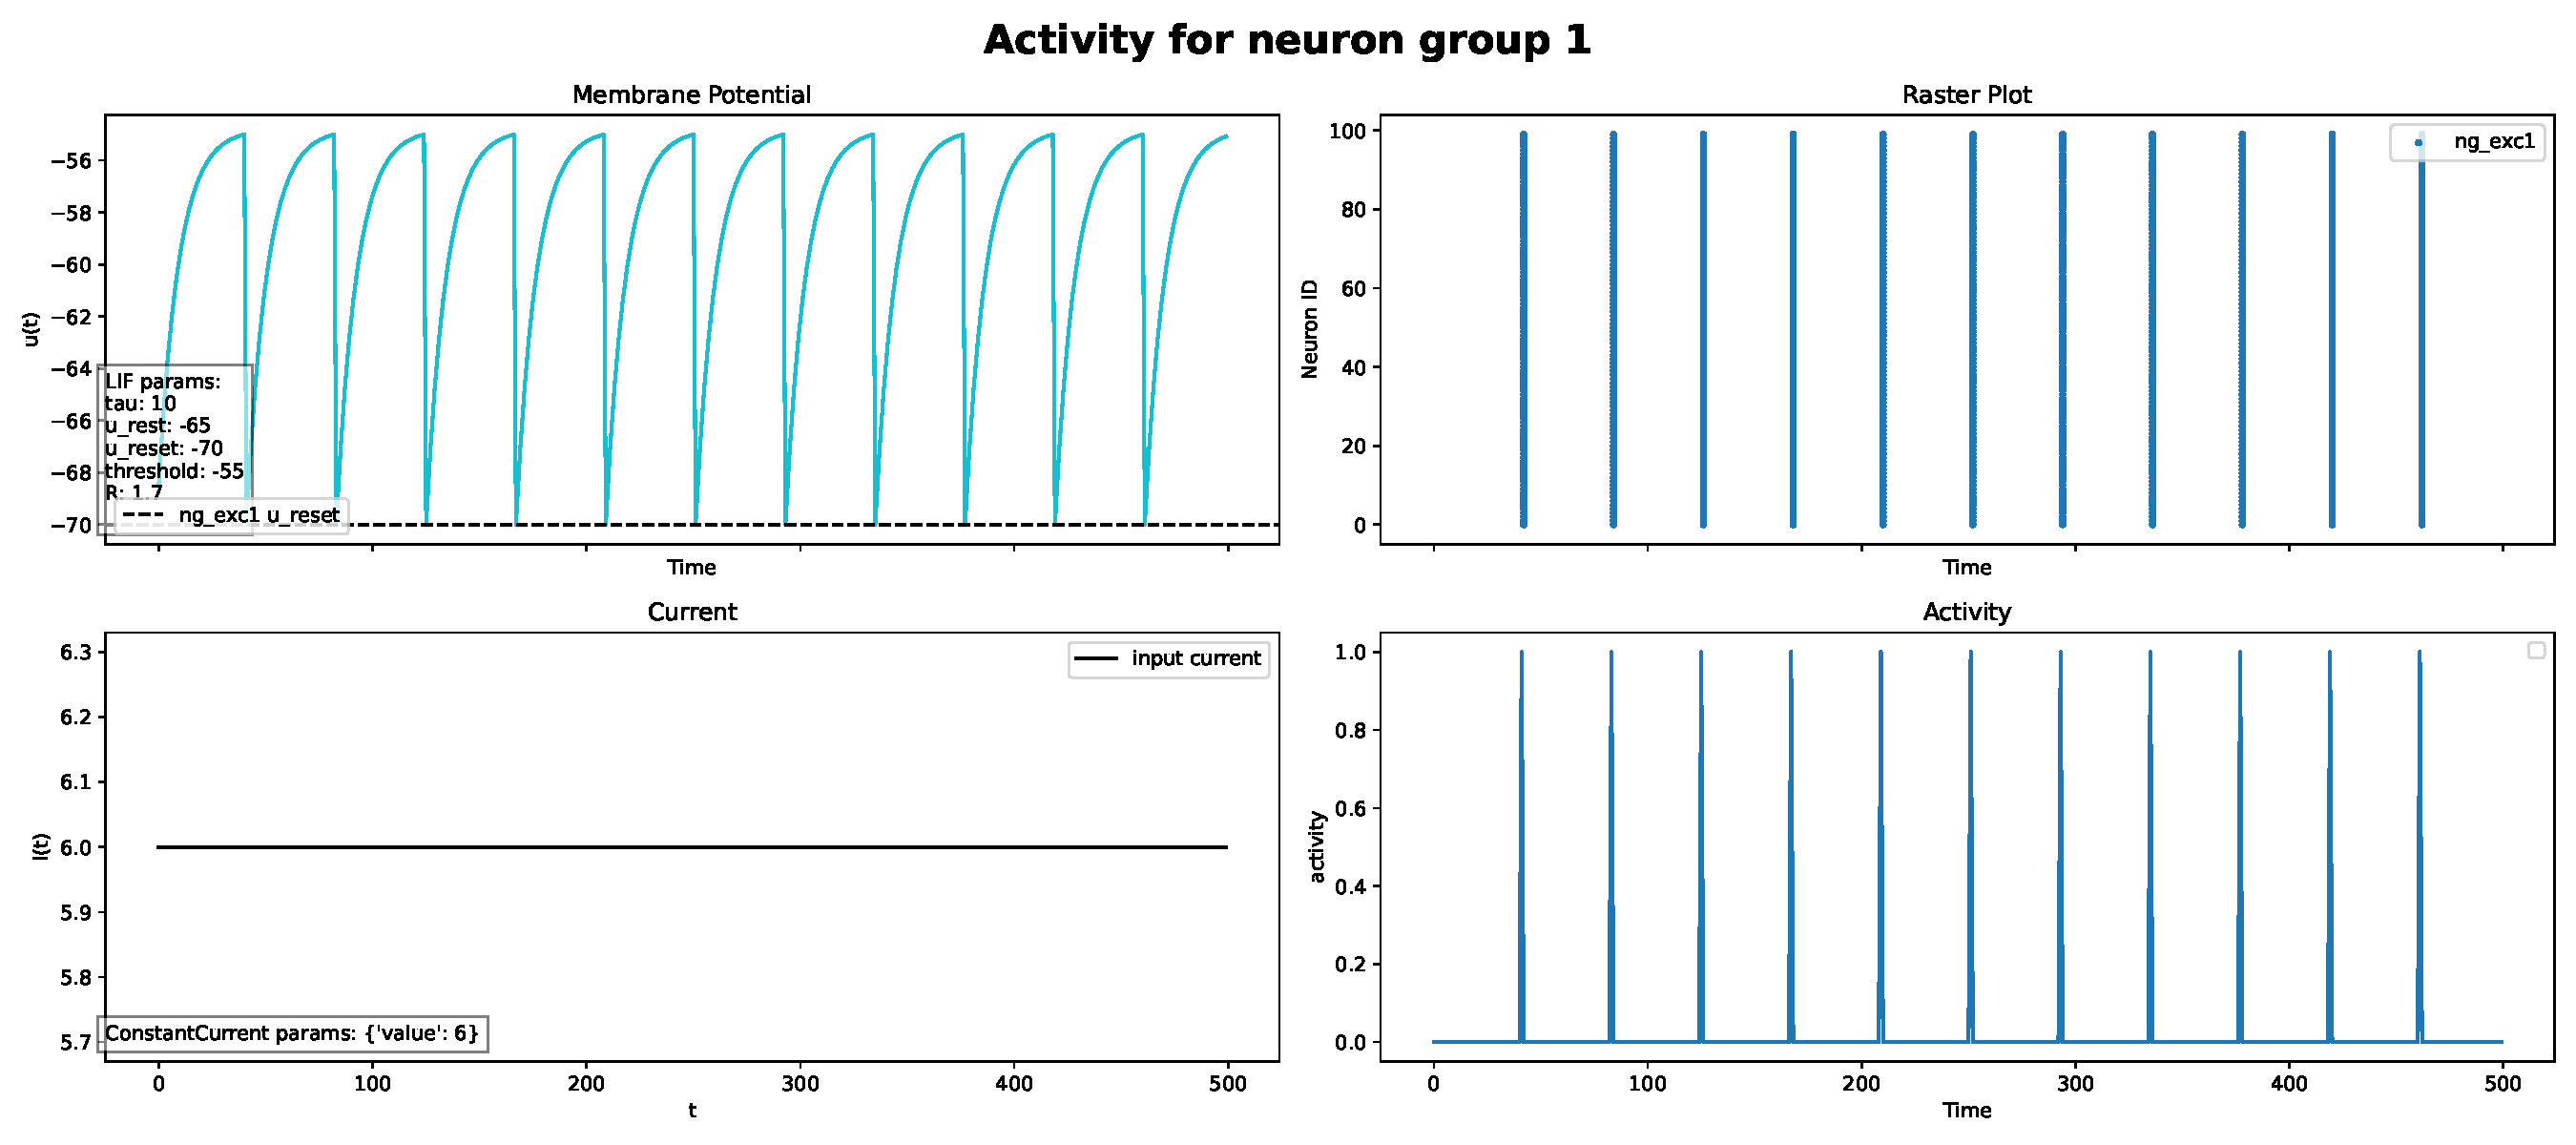
\includegraphics[width=0.9\textwidth]{plots/part1-Simple-ng-without-synapse.pdf} 
            \caption{جمعیت نورونی بدون سیناپس}
            \label{fig:part1-simple-ng}
        \end{figure}

        حال بیاید مقادیر اولیه نورون ها مانند اختلاف پتانسیل اولیه آن ها را تغییر دهیم تا رفتار آن ها را ببینیم. برای اینکار، اختلاف پتانسیل اولیه نورون ها را در حدود بازه ۶۷ با واریانس ۲ توزیع میکنیم. همانطور که در شکل
        \ref{fig:part1-simple-ng-u-init}
        نیز مشاهده می کنیم، نورون ها در ابتدا با یک اختلاف پتانسیل متفاوت شروع به فعالیت میکنند و از آنجا که جریان ورودی به آن ها نیز یکسان است، فواصل ضربه زدن خود را حفظ میکنند و با همان فواصل به ضربه زدن ادامه می دهند. در نتیجه فعالیت کلی جمعیت، به صورت دوره ای تکرار خواهد شد.
        \begin{figure}[!ht]
            \centering
            \includegraphics[width=0.9\textwidth]{plots/part1-Simple-ng-without-synapse-u\_init.pdf} 
            \caption{جمعیت نورونی بدون سیناپس: اختلاف پتانسیل اولیه متفاوت}
            \label{fig:part1-simple-ng-u-init}
        \end{figure}

        حال اگر به همین جمعیت یک جریان نویز دار اضافه کنیم چه اتفاقی می افتد؟ برای اینکار یک رفتار
        (\lr{Behavior})
        به نام 
        \texttt{NoiseCurrent}
        تعریف میکنیم که وظیفه آن اضافه کردن نویز به جریان نورون باشد. مقدار این نویز را یک جریان رندوم با میانگین ۰ و واریانس ۰.۱ قرار می دهیم. همانطور که در شکل 
        \ref{fig:part1-simple-ng-u-init-noise-curr}
        مشاهده میکنیم، به دلیل اضافه شدن نویز، الگوی فعالت نورون ها در بازه هایی که ضربه میزنند رفته رفته تغییر کرده و الگوی خود را از دست می دهند. هر چند اگر میزان این نویز خیلی زیاد باشد، می تواند برآیند جریان ورودی را زیاد کرده، به نحوی که رفتار نورون ها پس از مدتی مشابه شود.
        (شکل \ref{fig:part1-simple-ng-u-init-high-noise-curr})
        \begin{figure}[!ht]
            \centering
            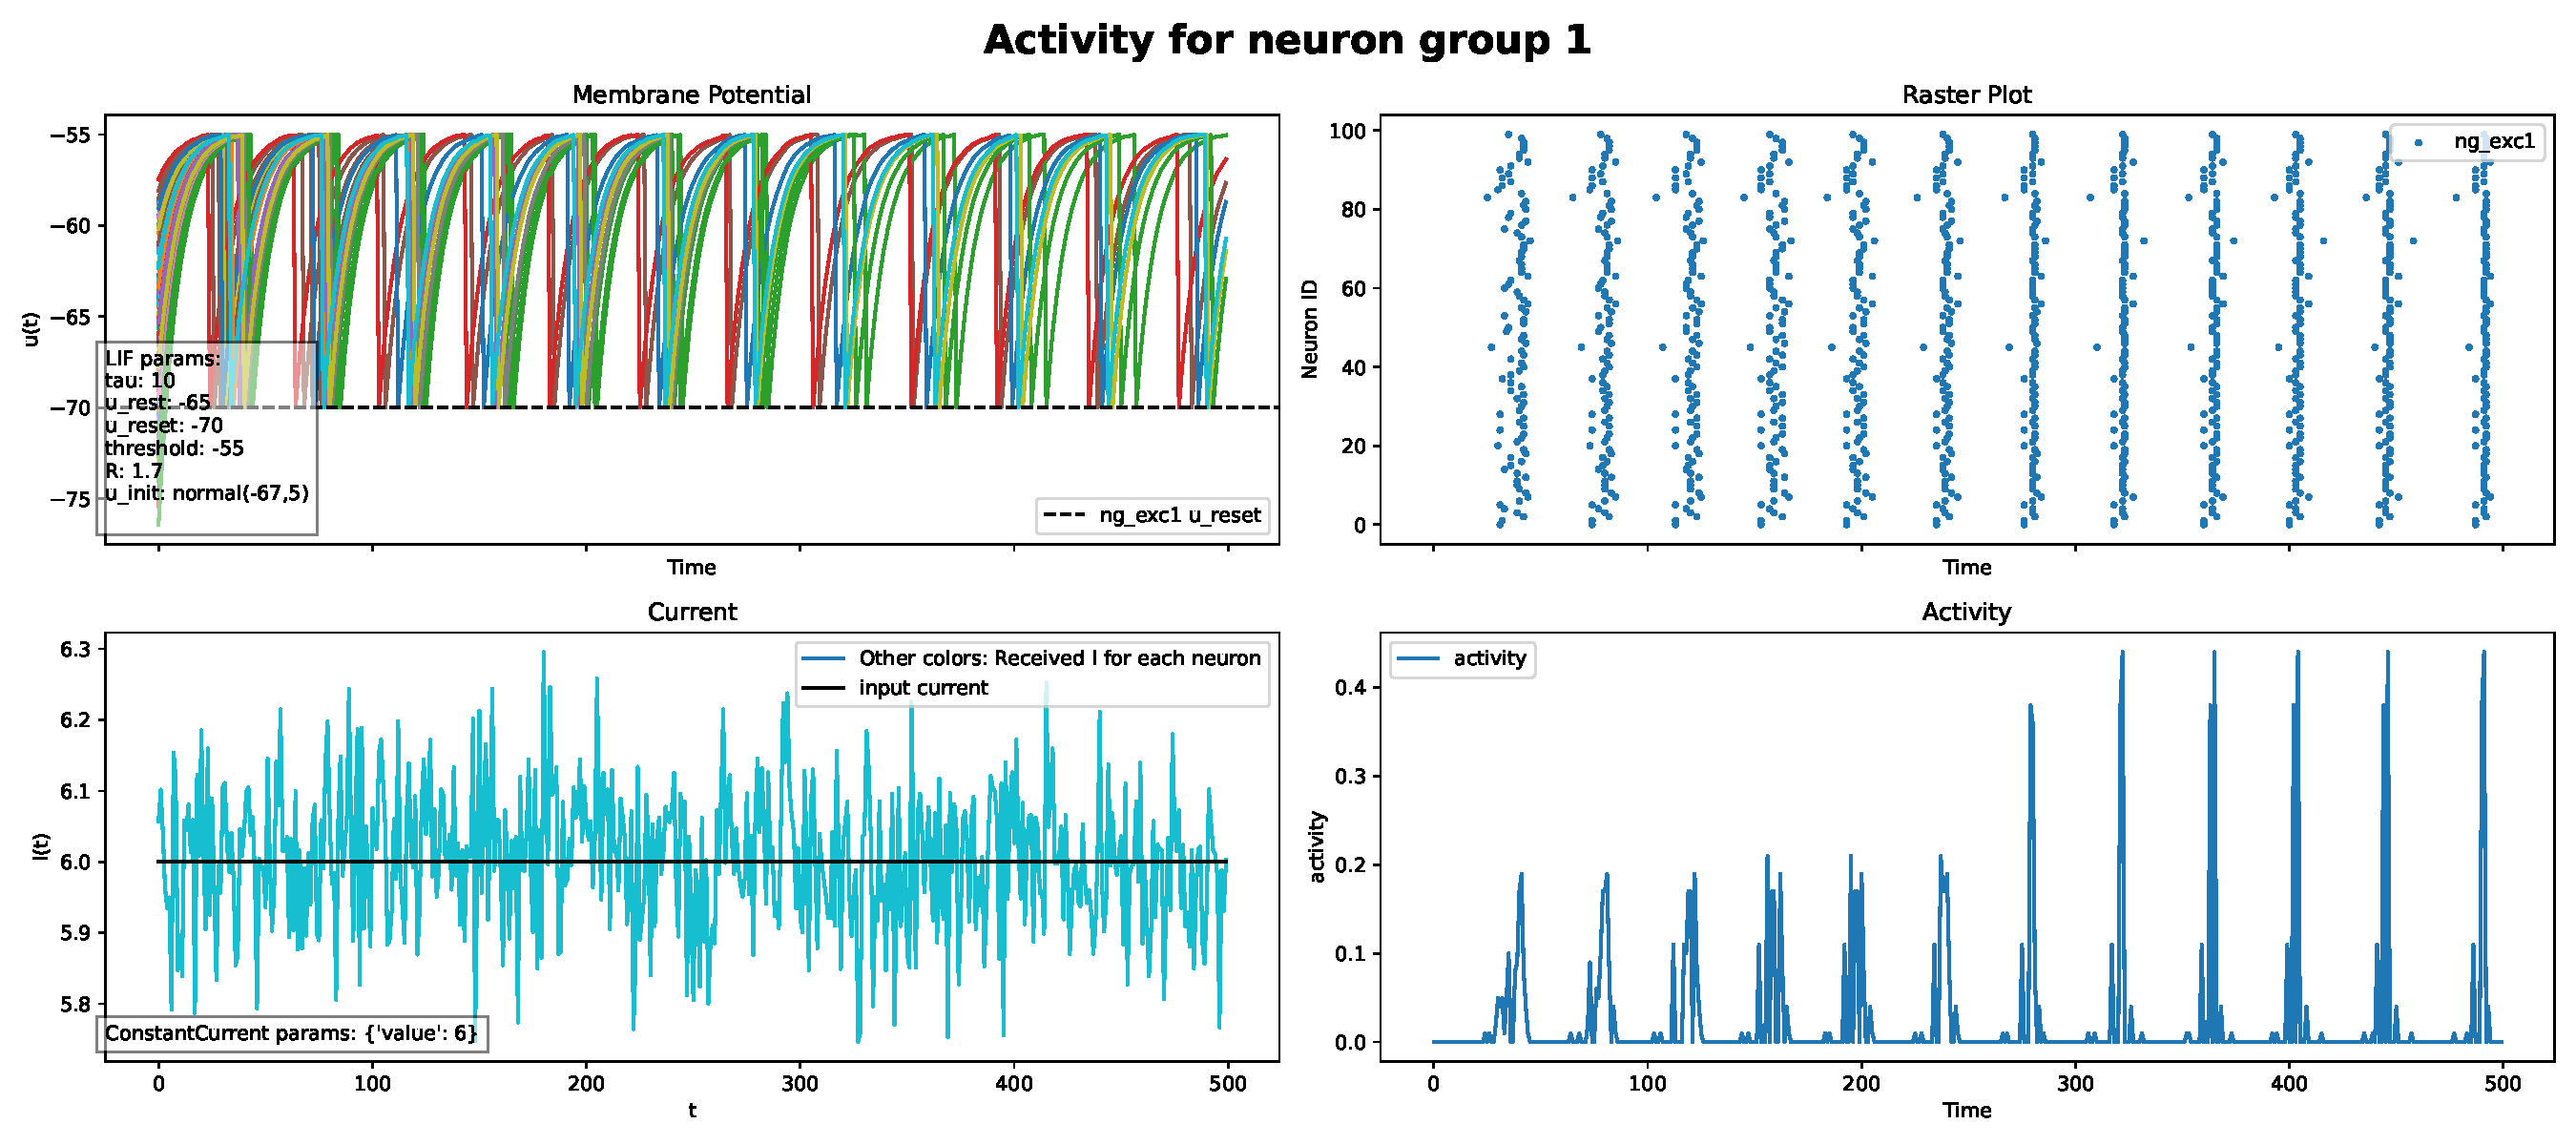
\includegraphics[width=0.9\textwidth]{plots/part1-Simple-ng-without-synapse-noise-curr.pdf} 
            \caption{جمعیت نورونی بدون سیناپس: اختلاف پتانسیل اولیه متفاوت و جریان نویزی}
            \label{fig:part1-simple-ng-u-init-noise-curr}
        \end{figure}
        \begin{figure}[!ht]
            \centering
            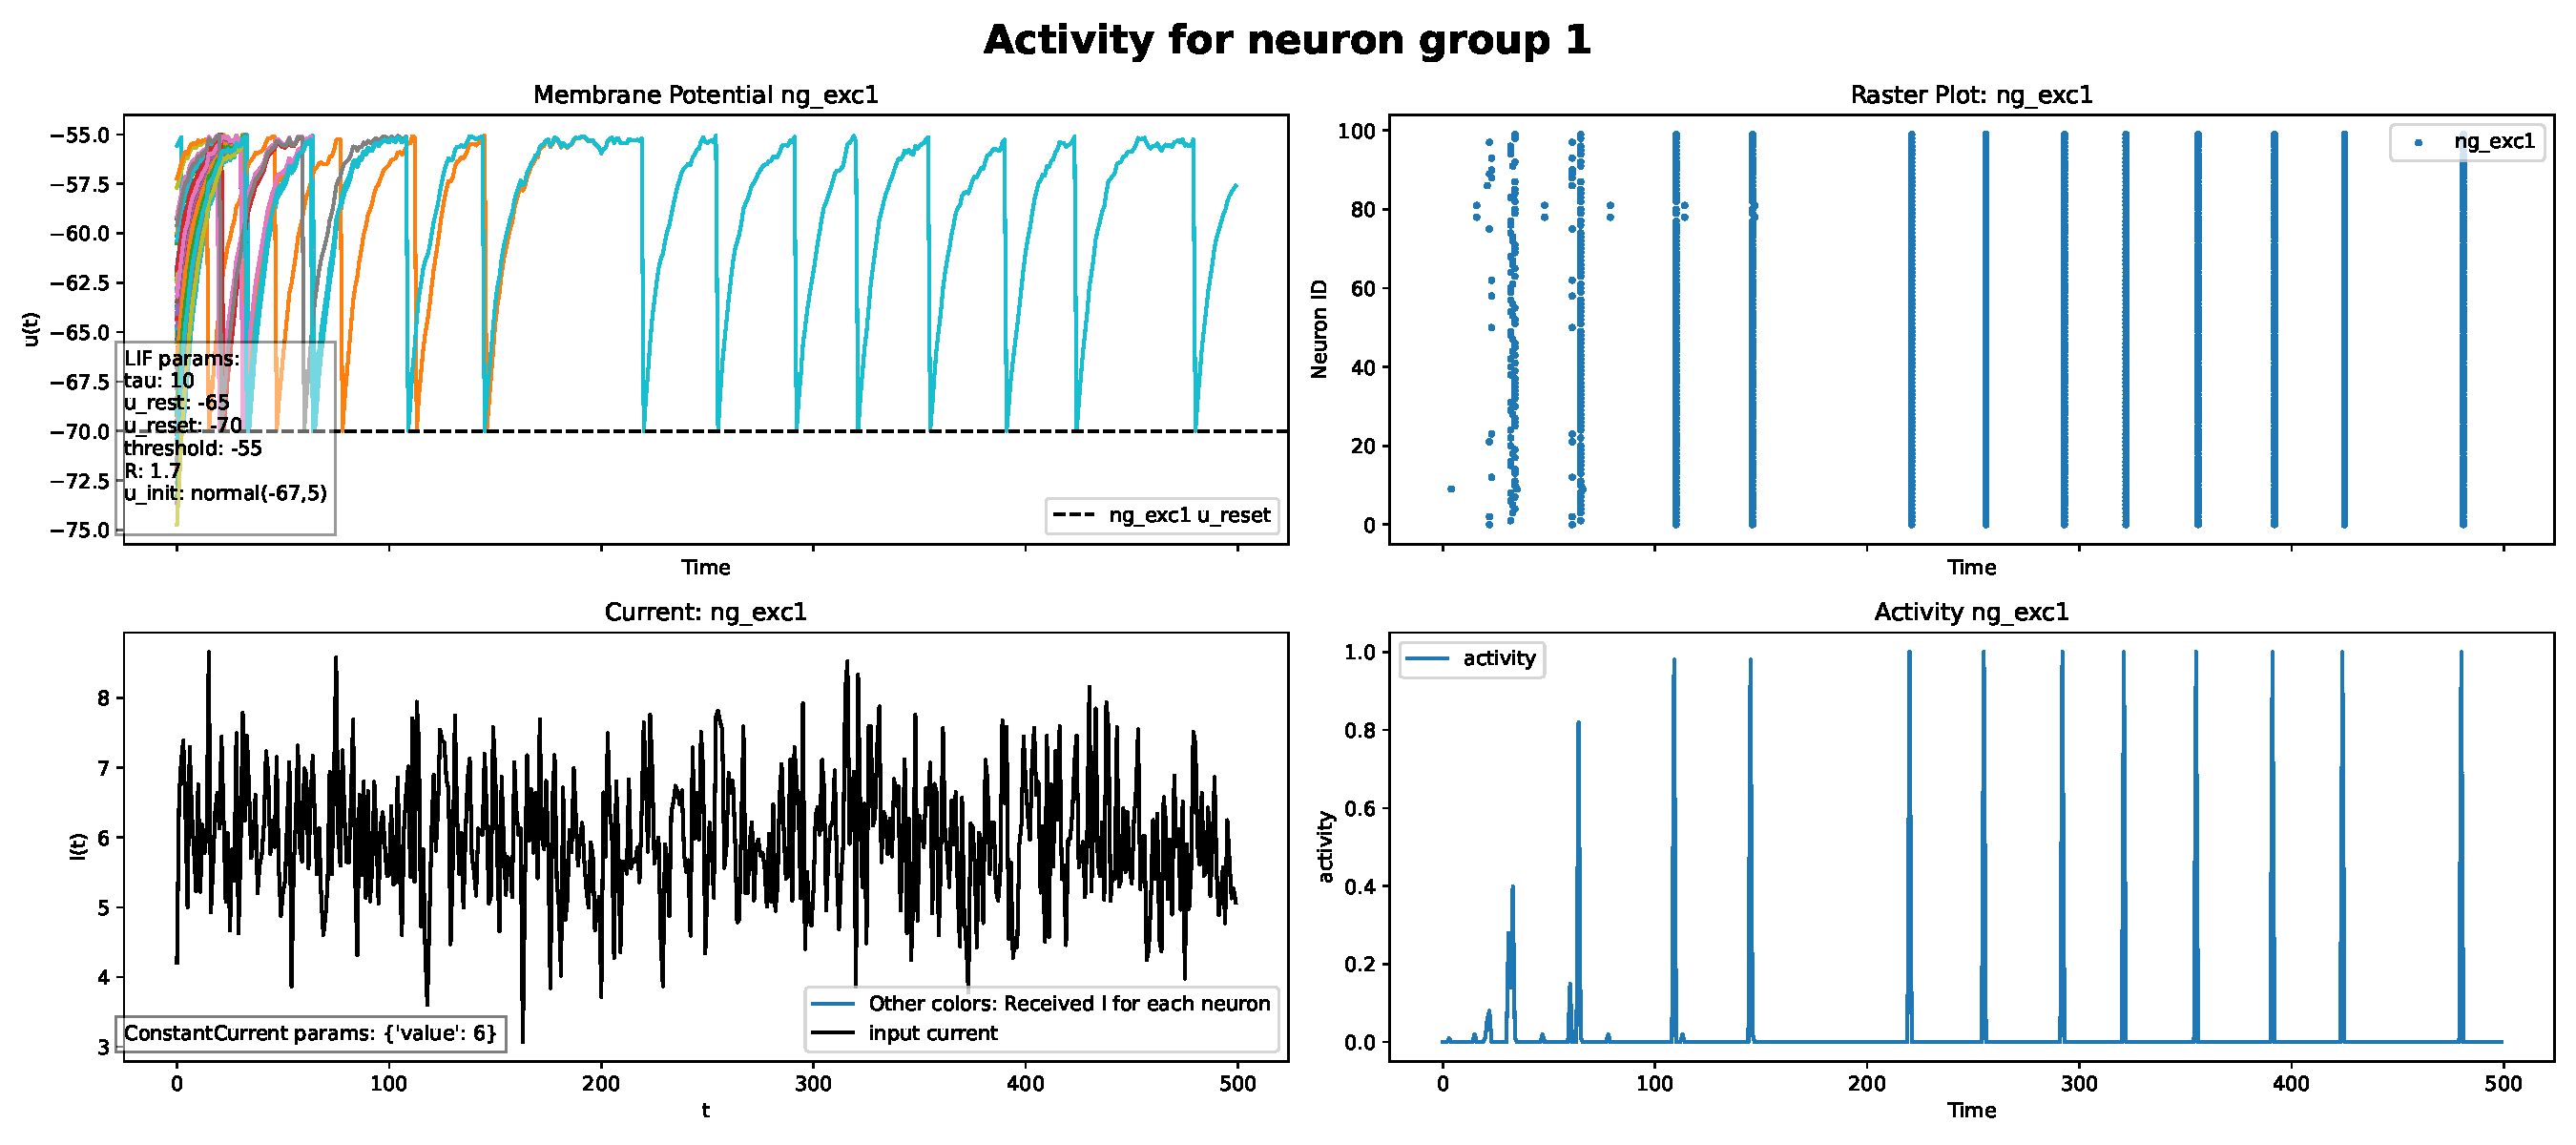
\includegraphics[width=0.9\textwidth]{plots/part1-Simple-ng-without-synapse-high-noise-curr.pdf} 
            \caption{جمعیت نورونی بدون سیناپس: اختلاف پتانسیل اولیه متفاوت و جریان نویزی زیاد}
            \label{fig:part1-simple-ng-u-init-high-noise-curr}
        \end{figure}

        حال فعالیت جمعیت نورونی را با جریان متفاوت برای هر نورون آزمایش میکنیم تا رفتار آن ها را بر این اساس نیز مشاهده کنیم. برای اینکار، جریان ورودی به جمعیت نورونی را با واریانس 
        $0.2$
        اضافه میکنیم. همانطور که در شکل 
        \ref{fig:part1-simple-ng-variance-curr}
        مشاهده میکنیم، تغییر دادن جریان ورودی به ازای هر نورون، زمان ضربه زدن هر نورون را از دیگری نسبت به حالت های قبل بیشتر متفاوت می کند و در نتیجه، پراکندگی زمان فعالیت نورون ها بیشتر می شود. همچنین اضافه کردن واریانس بیشتر میتواند پراکندگی را آنقدر افزایش دهد تا تشخیص یک الگو برای زمان ضربه زدن نورون ها بسیار سخت تر شود
        (شکل \ref{fig:part1-simple-ng-high-variance-curr})
        \begin{figure}[!ht]
            \centering
            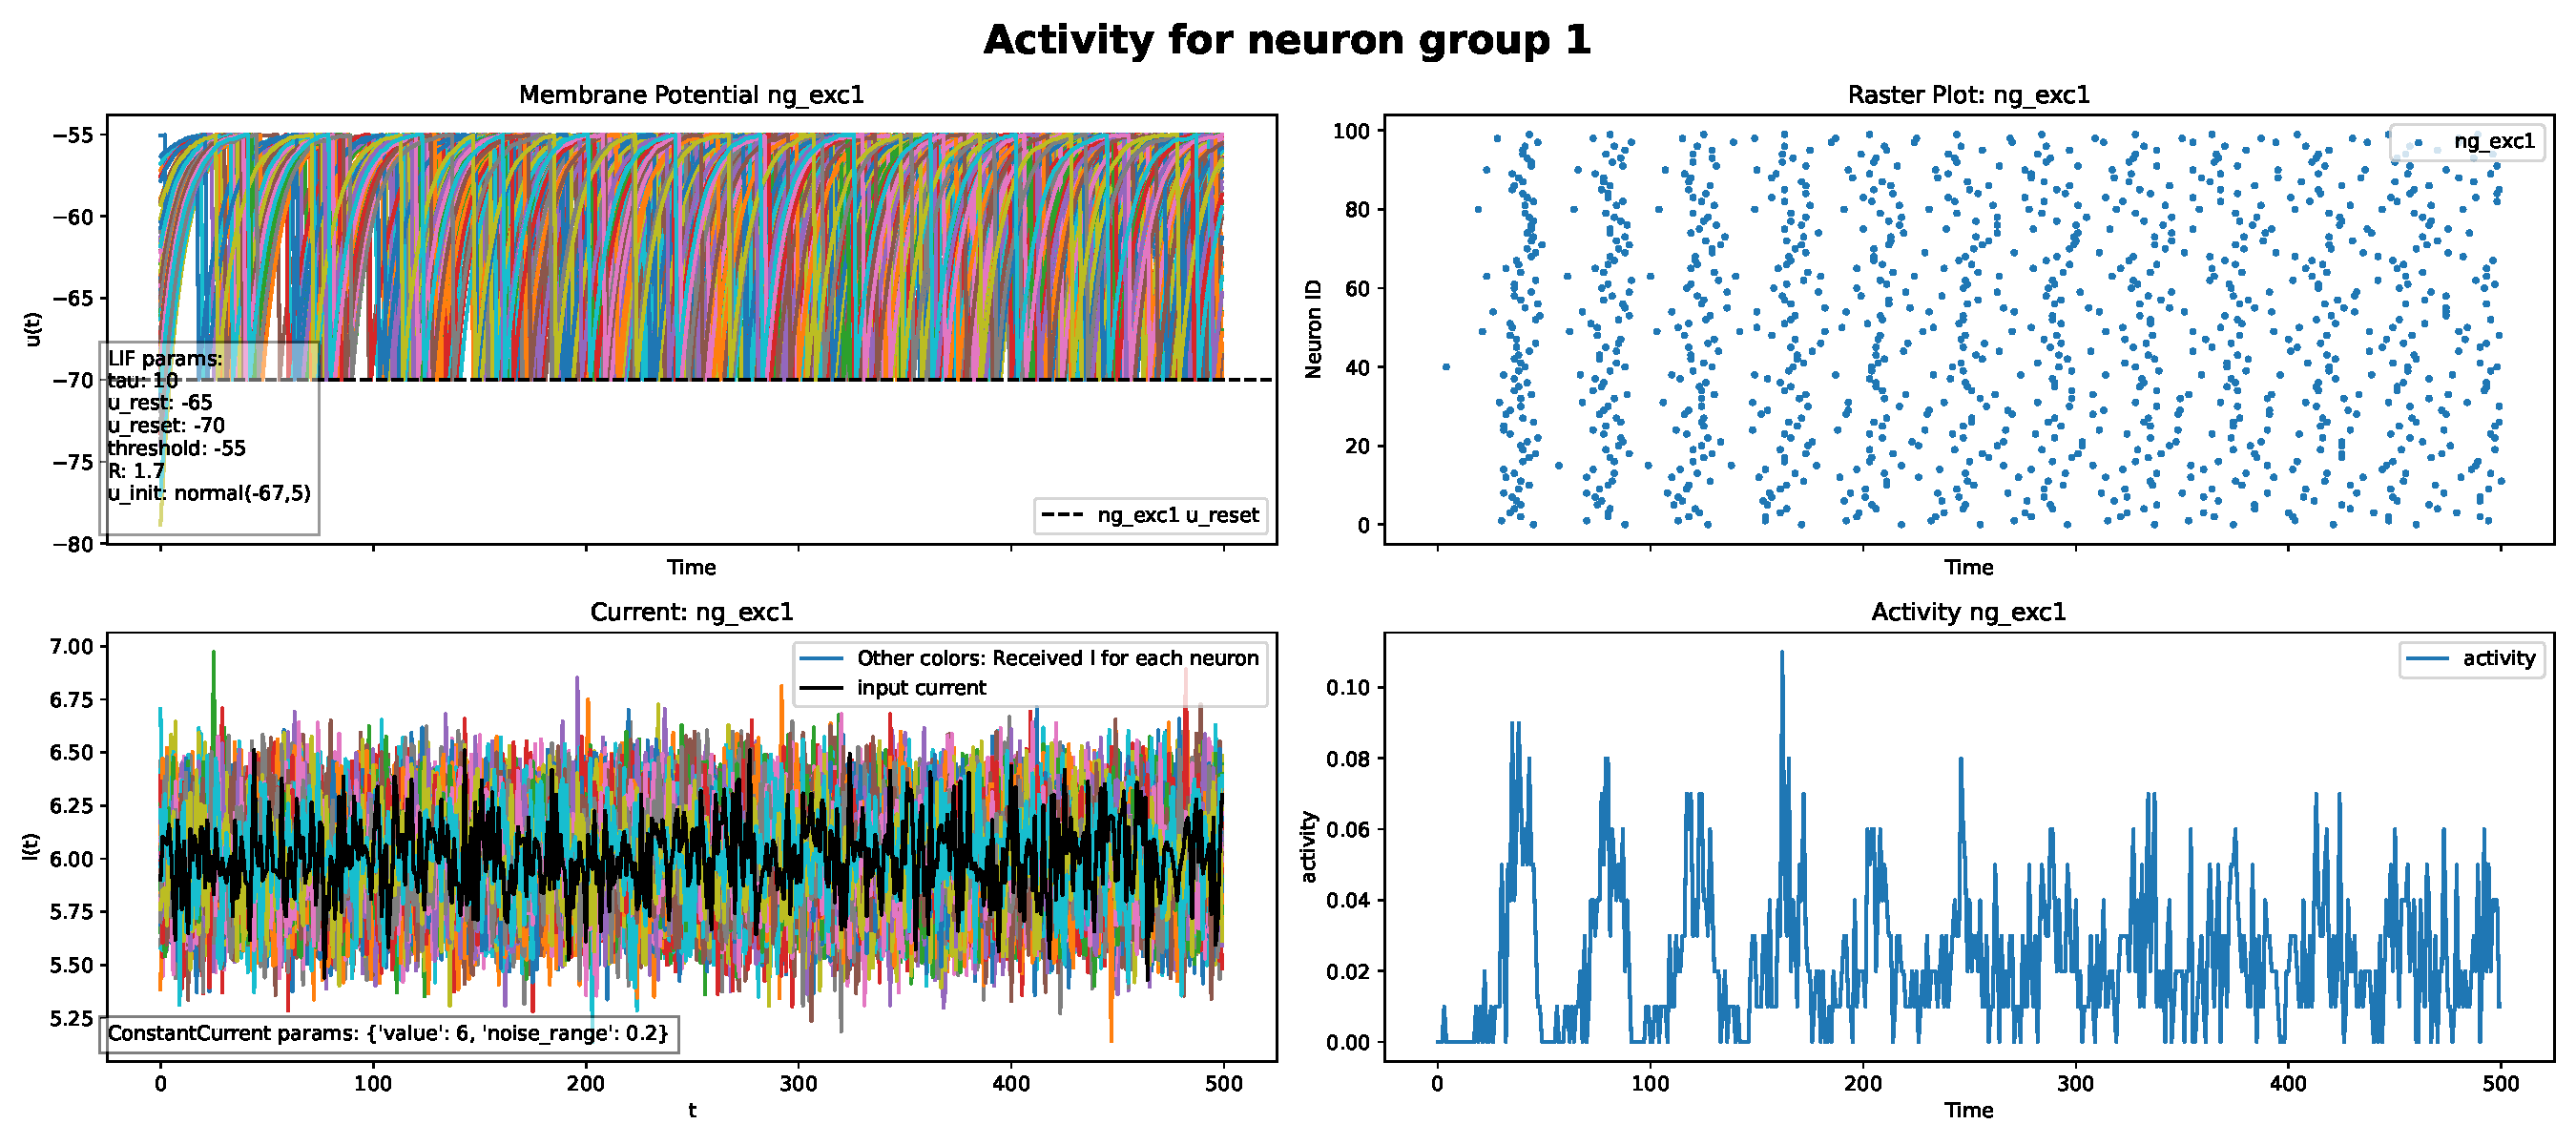
\includegraphics[width=0.9\textwidth]{plots/part1-Simple-ng-without-synapse-variance-curr.pdf} 
            \caption{جمعیت نورونی بدون سیناپس: جریان ورودی متفاوت}
            \label{fig:part1-simple-ng-variance-curr}
        \end{figure}
        \begin{figure}[!ht]
            \centering
            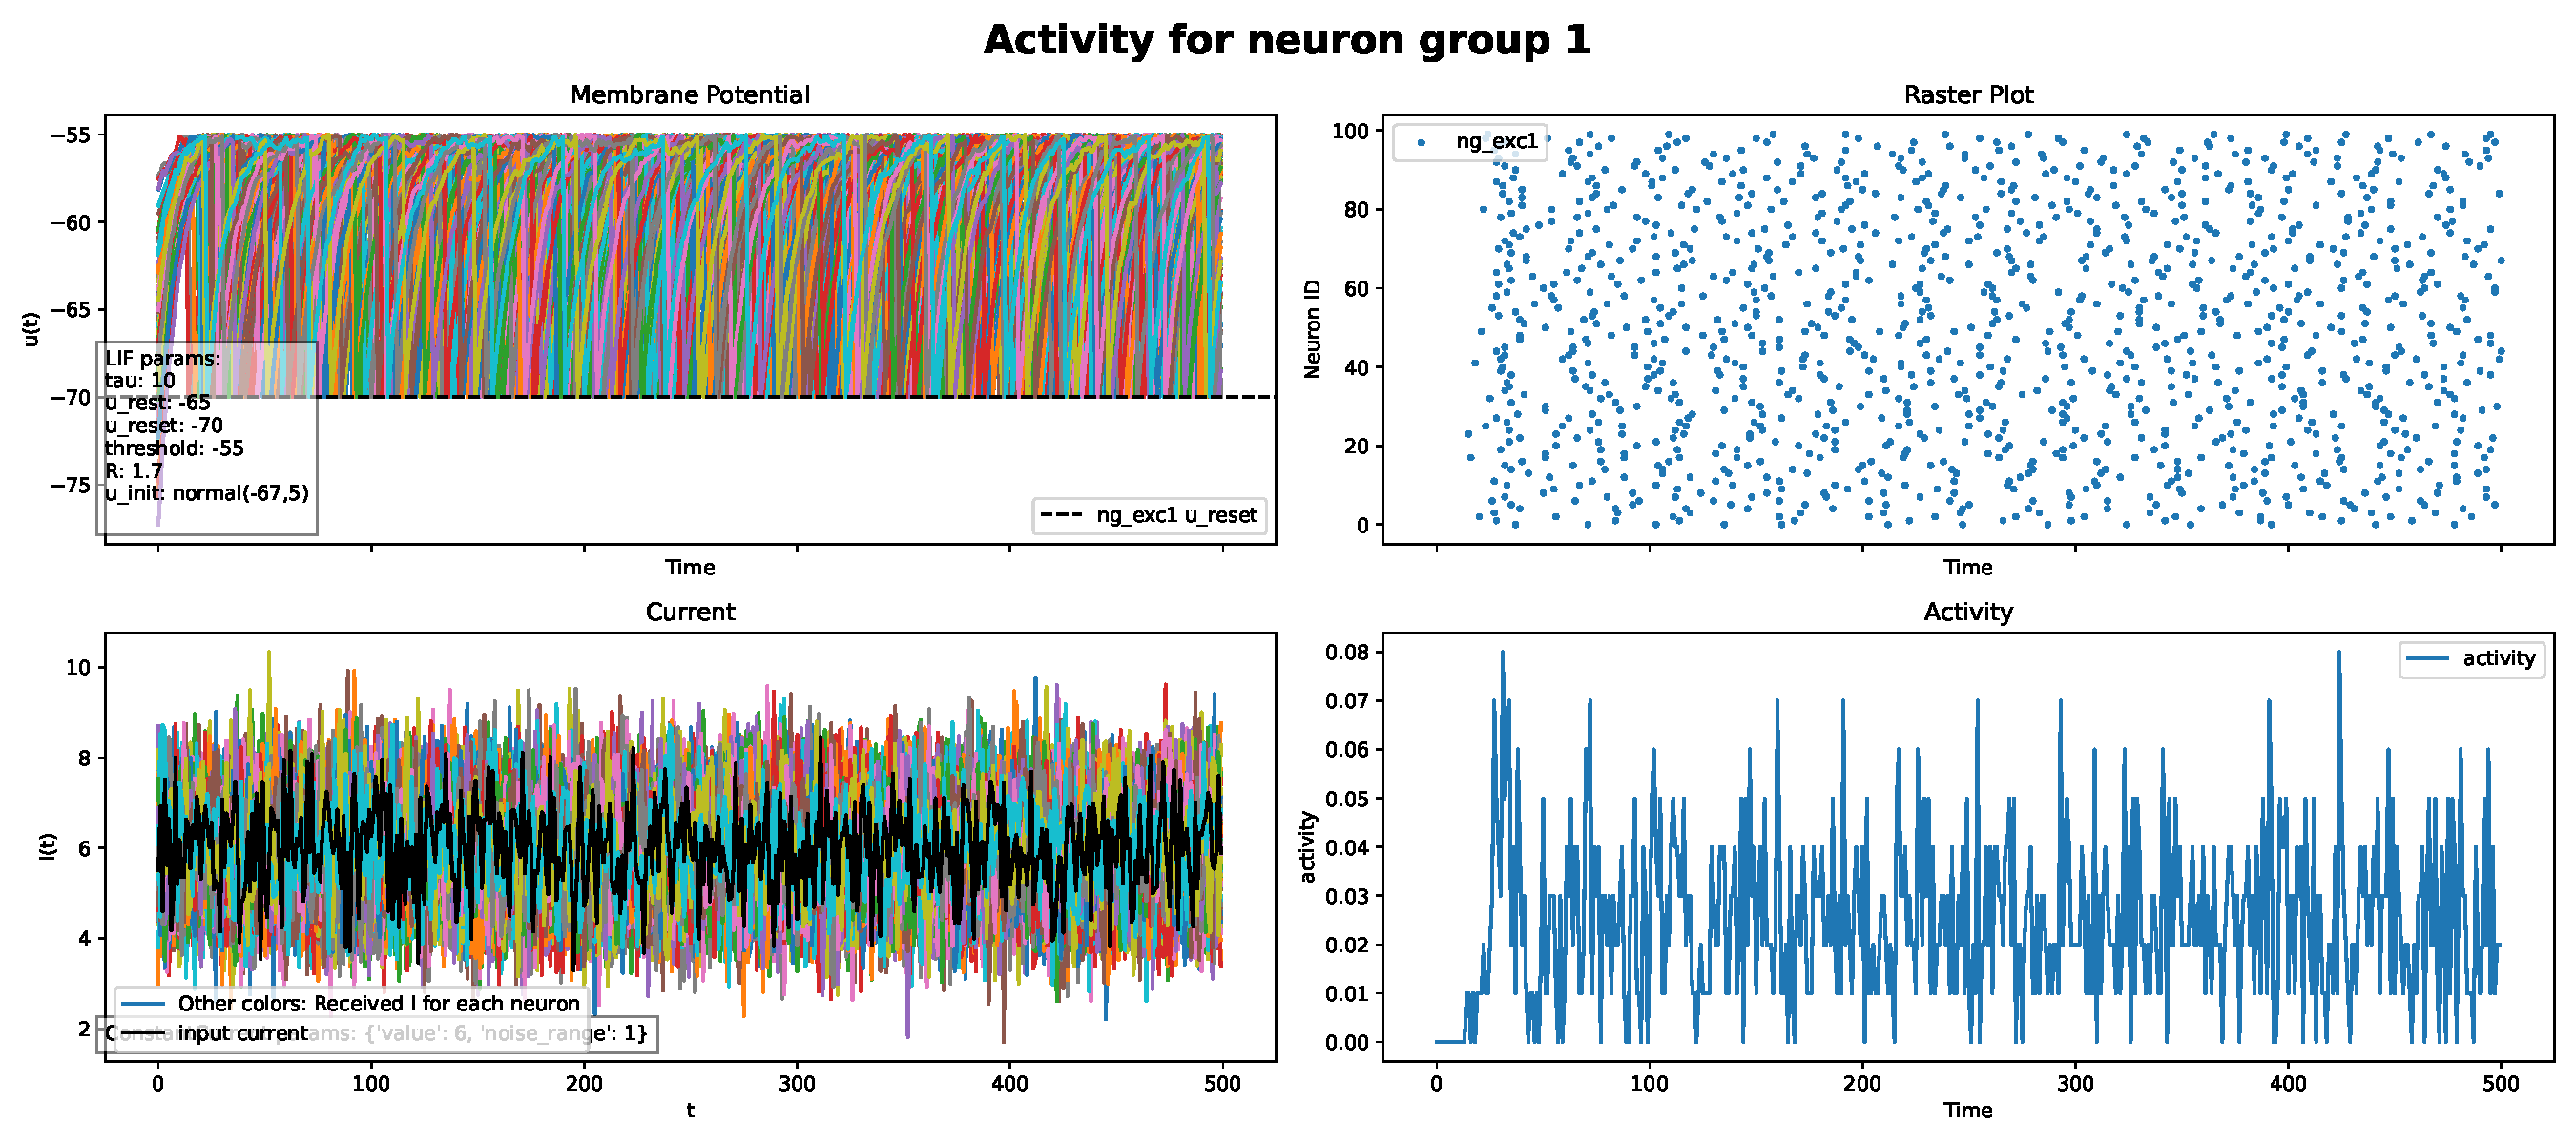
\includegraphics[width=0.9\textwidth]{plots/part1-Simple-ng-without-synapse-high-variance-curr.pdf} 
            \caption{جمعیت نورونی بدون سیناپس: جریان ورودی با تفاوت زیاد}
            \label{fig:part1-simple-ng-high-variance-curr}
        \end{figure}

        \subsubsection*{جمعیت نورونی به همراه سیناپس}
        حال که تاثیر انواع متفاوت جریان را بر یک جمعیت نورونی بررسی کردیم، به سراغ اضافه کردن سیناپس به آن میرویم. برای سادگی، سیناپس را با الگوی ارتباط کامل
        \footnote{\lr{full connectivity}}
        بررسی میکنیم و بررسی الگو های دیگر را به بخش دوم پروژه واگذار میکنیم. در ابتدا نیز وزن های سیناپسی را کامل یکسان با
        $j_0=5$ و $\sigma=0$
        در نظر میگیریم و سپس به آن واریانس اضافه میکنیم. همانطور که در شکل
        \ref{fig:part1-simple-ng-with-synapse}
        ملاحظه میکنیم، در یک جمعیت نورونی به همراه سیناپس داخلی، که نورون ها نیز در زمان اولیه اختلاف پتانسیل یکسانی دارند، رفتار جمعیت همانند هنگامی است که سیناپس وجود نداشته باشد. این به این دلیل است که در این حالت، قبل از اولین ضربه سیناپس تاثیری ندارد و رفتار نورون  همانند جمعیت بدون سیناپس با جریان ورودی ثابت است. از این رو اختلاف پتانسیل نورون ها به طور همزمان افزایش می یابد تا هنگامی که به  آستانه رسیده و نورون ها همزمان ضربه می زنند. در این لحظه، بلافاصله جریان سیناپسی نیز به جریان دریافتی نورون اضافه می شود و از آنجا که سیناپس ارتباط کامل است، زمان ضربه زدن نورون ها تغییری پیدا نمی کند.
        \begin{figure}[!ht]
            \centering
            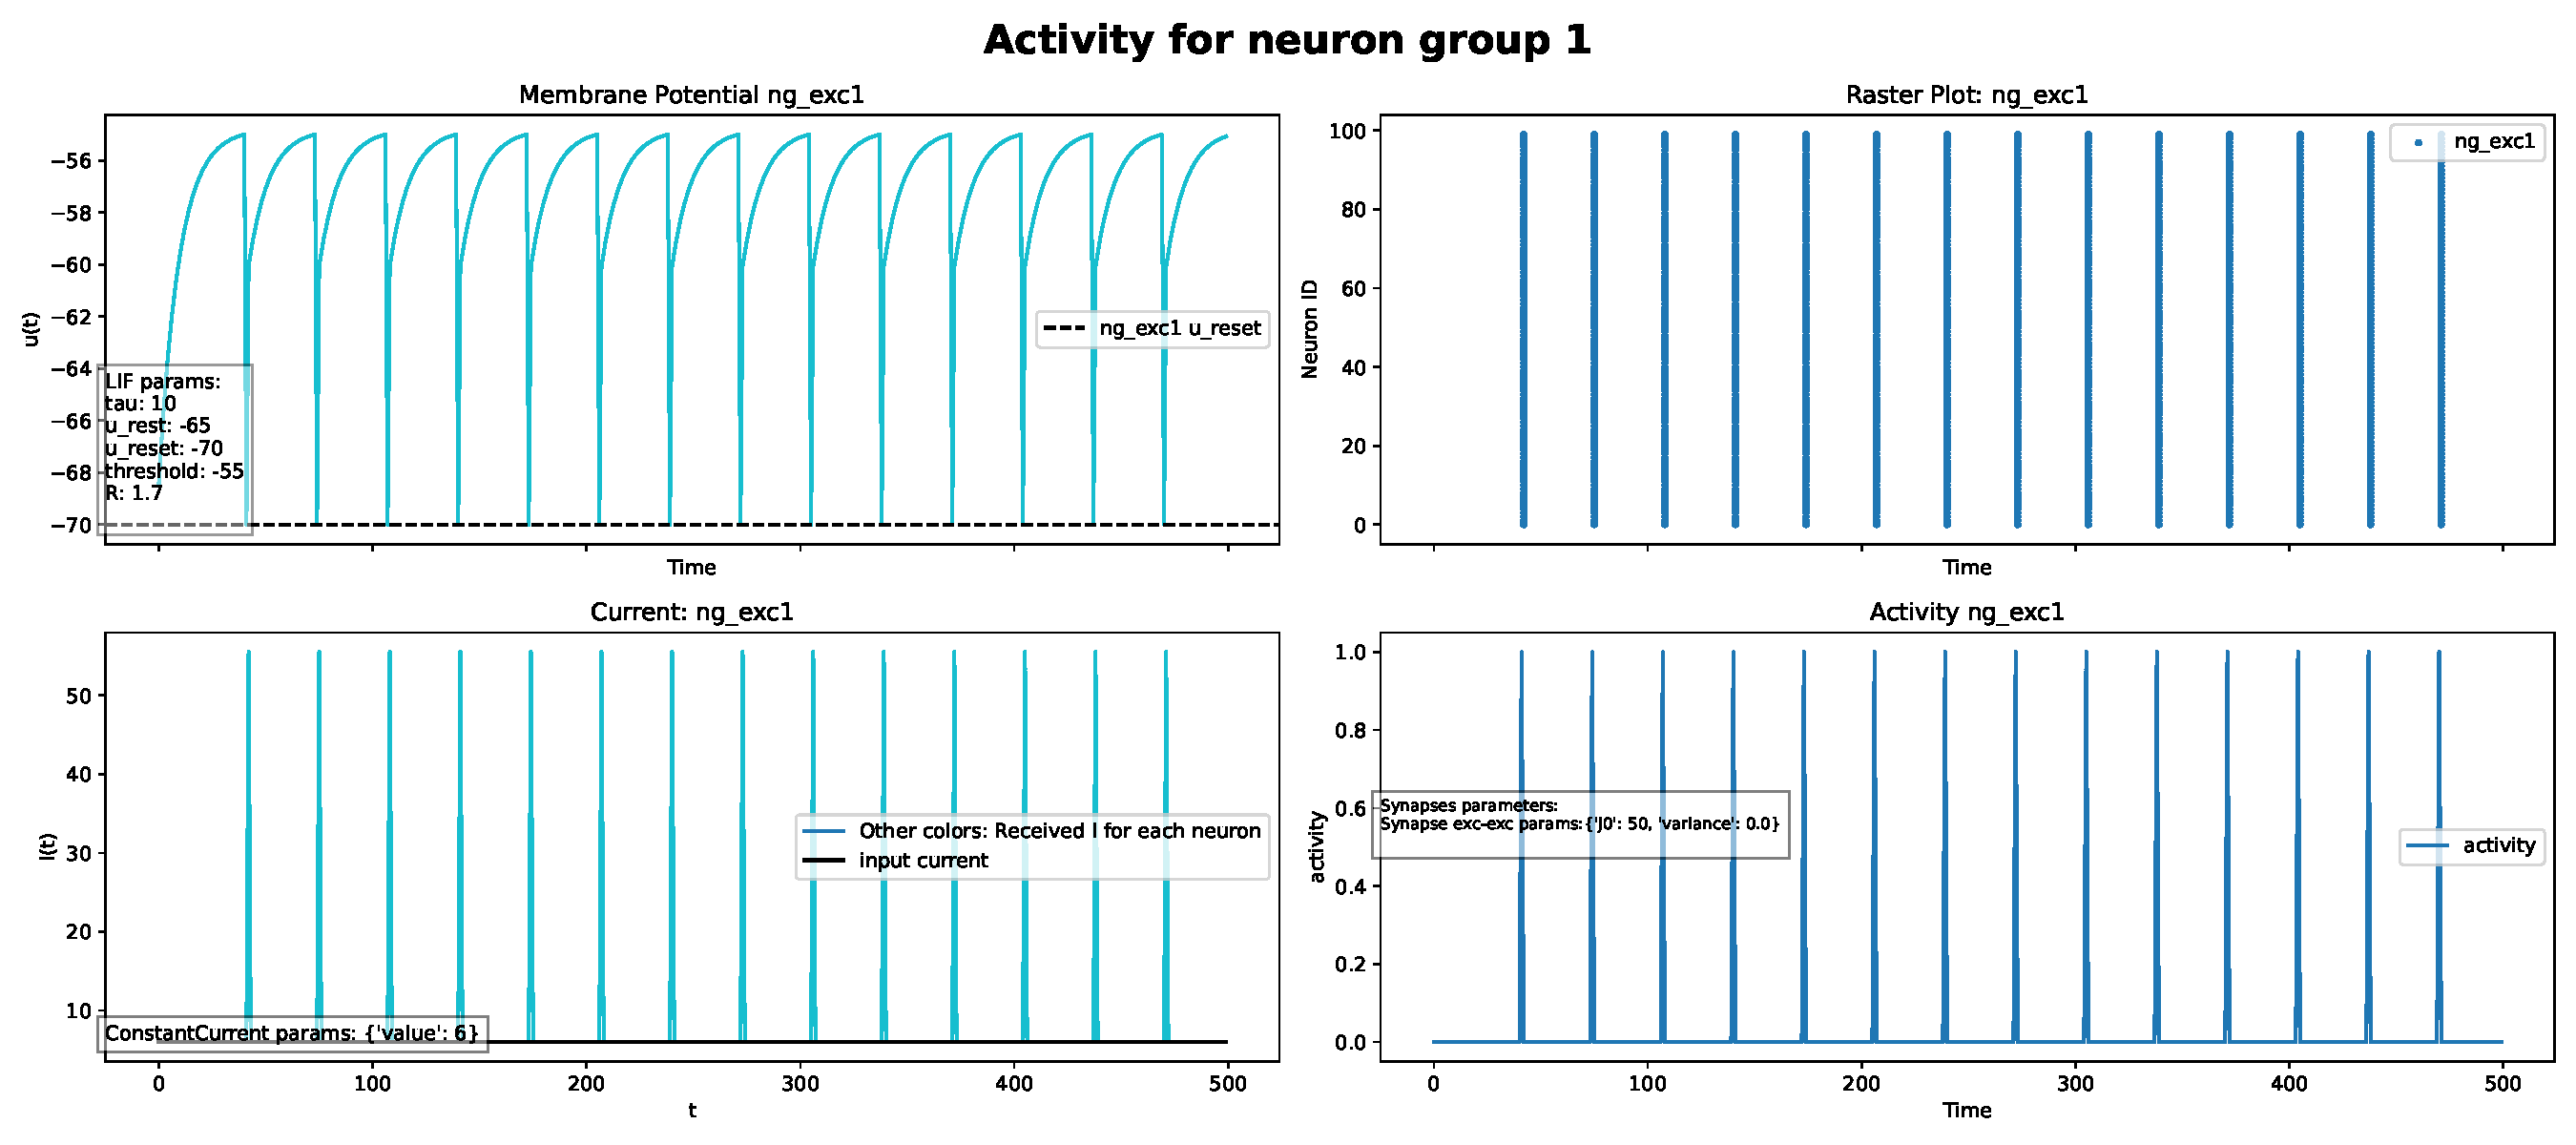
\includegraphics[width=0.9\textwidth]{plots/part1-Simple-ng-with-synapse.pdf} 
            \caption{جمعیت نورونی با سیناپس: جریان ثابت}
            \label{fig:part1-simple-ng-with-synapse}
        \end{figure}

        حال اگر اختلاف پتانسیل اولیه نورون ها را متفاوت مقدار دهی کنیم، مطابق شکل
        \ref{fig:part1-simple-ng-with-synapse-u-init}
        میبینیم که زمان ضربه زدن نورون ها متفاوت می شود.هر چند پس از مدتی، به دلیل اضافه شدن جریان سیناپسی به جریان ورودی نورون و درنتیجه افزایش یافتن جریان دریافتی نورون، این اختلاف زمانی ضربه ها نیز کمتر می شود. افزایش مقدار 
        $j_0$ 
        به ۱۰ نیز زمان این همگرایی را سریع تر می کند.
        (شکل \ref{fig:part1-simple-ng-with-synapse-u-init-high-j})
        \begin{figure}[!ht]
            \centering
            \includegraphics[width=0.9\textwidth]{plots/part1-Simple-ng-with-synapse-u\_init.pdf} 
            \caption{جمعیت نورونی با سیناپس: اختلاف پتانسیل اولیه متفاوت}
            \label{fig:part1-simple-ng-with-synapse-u-init}
        \end{figure}
        \begin{figure}[!ht]
            \centering
            \includegraphics[width=0.9\textwidth]{plots/part1-Simple-ng-with-synapse-u\_init-high\_j.pdf} 
            \caption{جمعیت نورونی با سیناپس: اختلاف پتانسیل اولیه متفاوت و وزن های بیشتر}
            \label{fig:part1-simple-ng-with-synapse-u-init-high-j}
        \end{figure}

        حال واریانس وزن های سیناپسی را از ۰ بیشتر میکنیم، تا تاثیر این پارامتر را بر روی رفتار جمعیت ملاحظه کنیم. انتظار داریم که افزودن پراکندگی به وزن ها باعث پراکندگی زمان ضربه زدن نورون ها نیز بشود. شکل 
        \ref{fig:part1-simple-ng-with-synapse-u_init-variance}
        این موضوع را تایید میکند و ملاظحه می شود که فعالیت نورون ها مانند شکل قبل همگرا نشده و بالا و پایین می شود
        (در نهایت بین مقادیر ۰.۶ و ۰.۸ نوسان می کند.)
        هرچند در کل تاثیر این پارامتر نسبت به پارامتر دیگر چندان زیاد نیست.
        
        \begin{figure}[!ht]
            \centering
            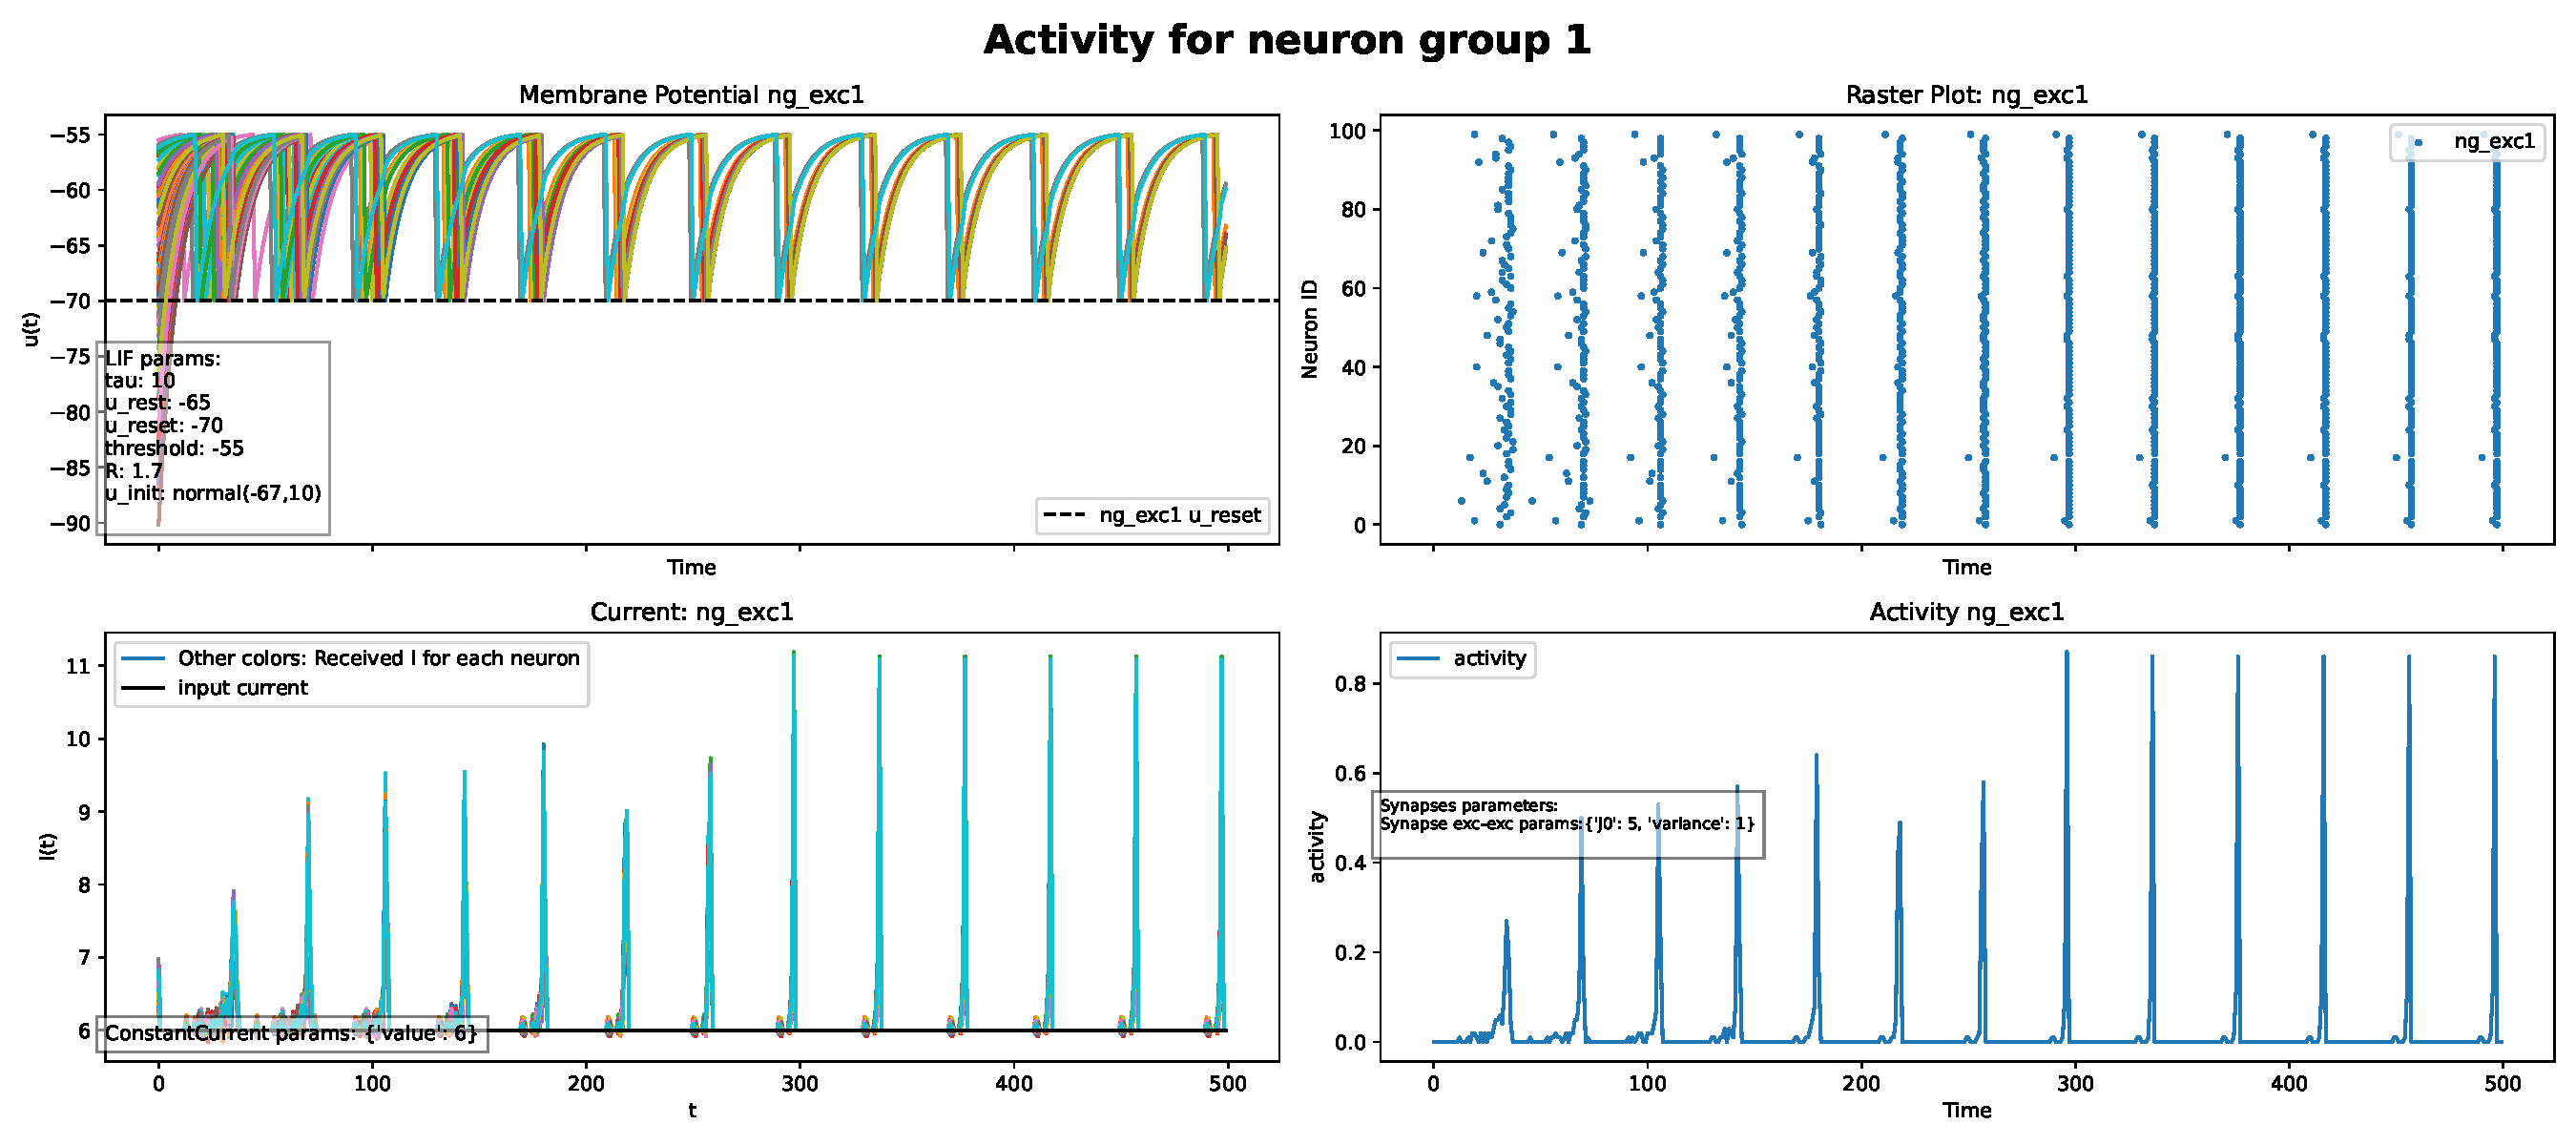
\includegraphics[width=0.9\textwidth]{plots/part1-Simple-ng-with-synapse-u_init-variance.pdf} 
            \caption{جمعیت نورونی با سیناپس: اختلاف پتانسیل اولیه متفاوت و وزن با واریانس بیشتر}
            \label{fig:part1-simple-ng-with-synapse-u_init-variance}
        \end{figure}
        بعد از بررسی پارامتر های سیناپس، نوبت به بررسی تاثیر جریان بر روی سیناپس می رسد. مطابق زیربخش قبل، در ابتدا رفتار جمعیت را با جریان نویزی یکسان برای همه نورون ها بررسی میکنیم. همانطور که در شکل
        \ref{fig:part1-simple-ng-with-synapse-noise-curr}
        مشاهده می شود، در ابتدا، زمان ضربه زدن نورون ها با یکدیگر متفاوت است و پس از مدتی این تفاوت کاهش یافته و همگرا می شود به طور که در نمودار فعالیت مشاهده می کنیم که ابتدا فعالیت نورونی حدود ۰ بوده و در نهایت به ۱ می رسد.
        \begin{figure}[!ht]
            \centering
            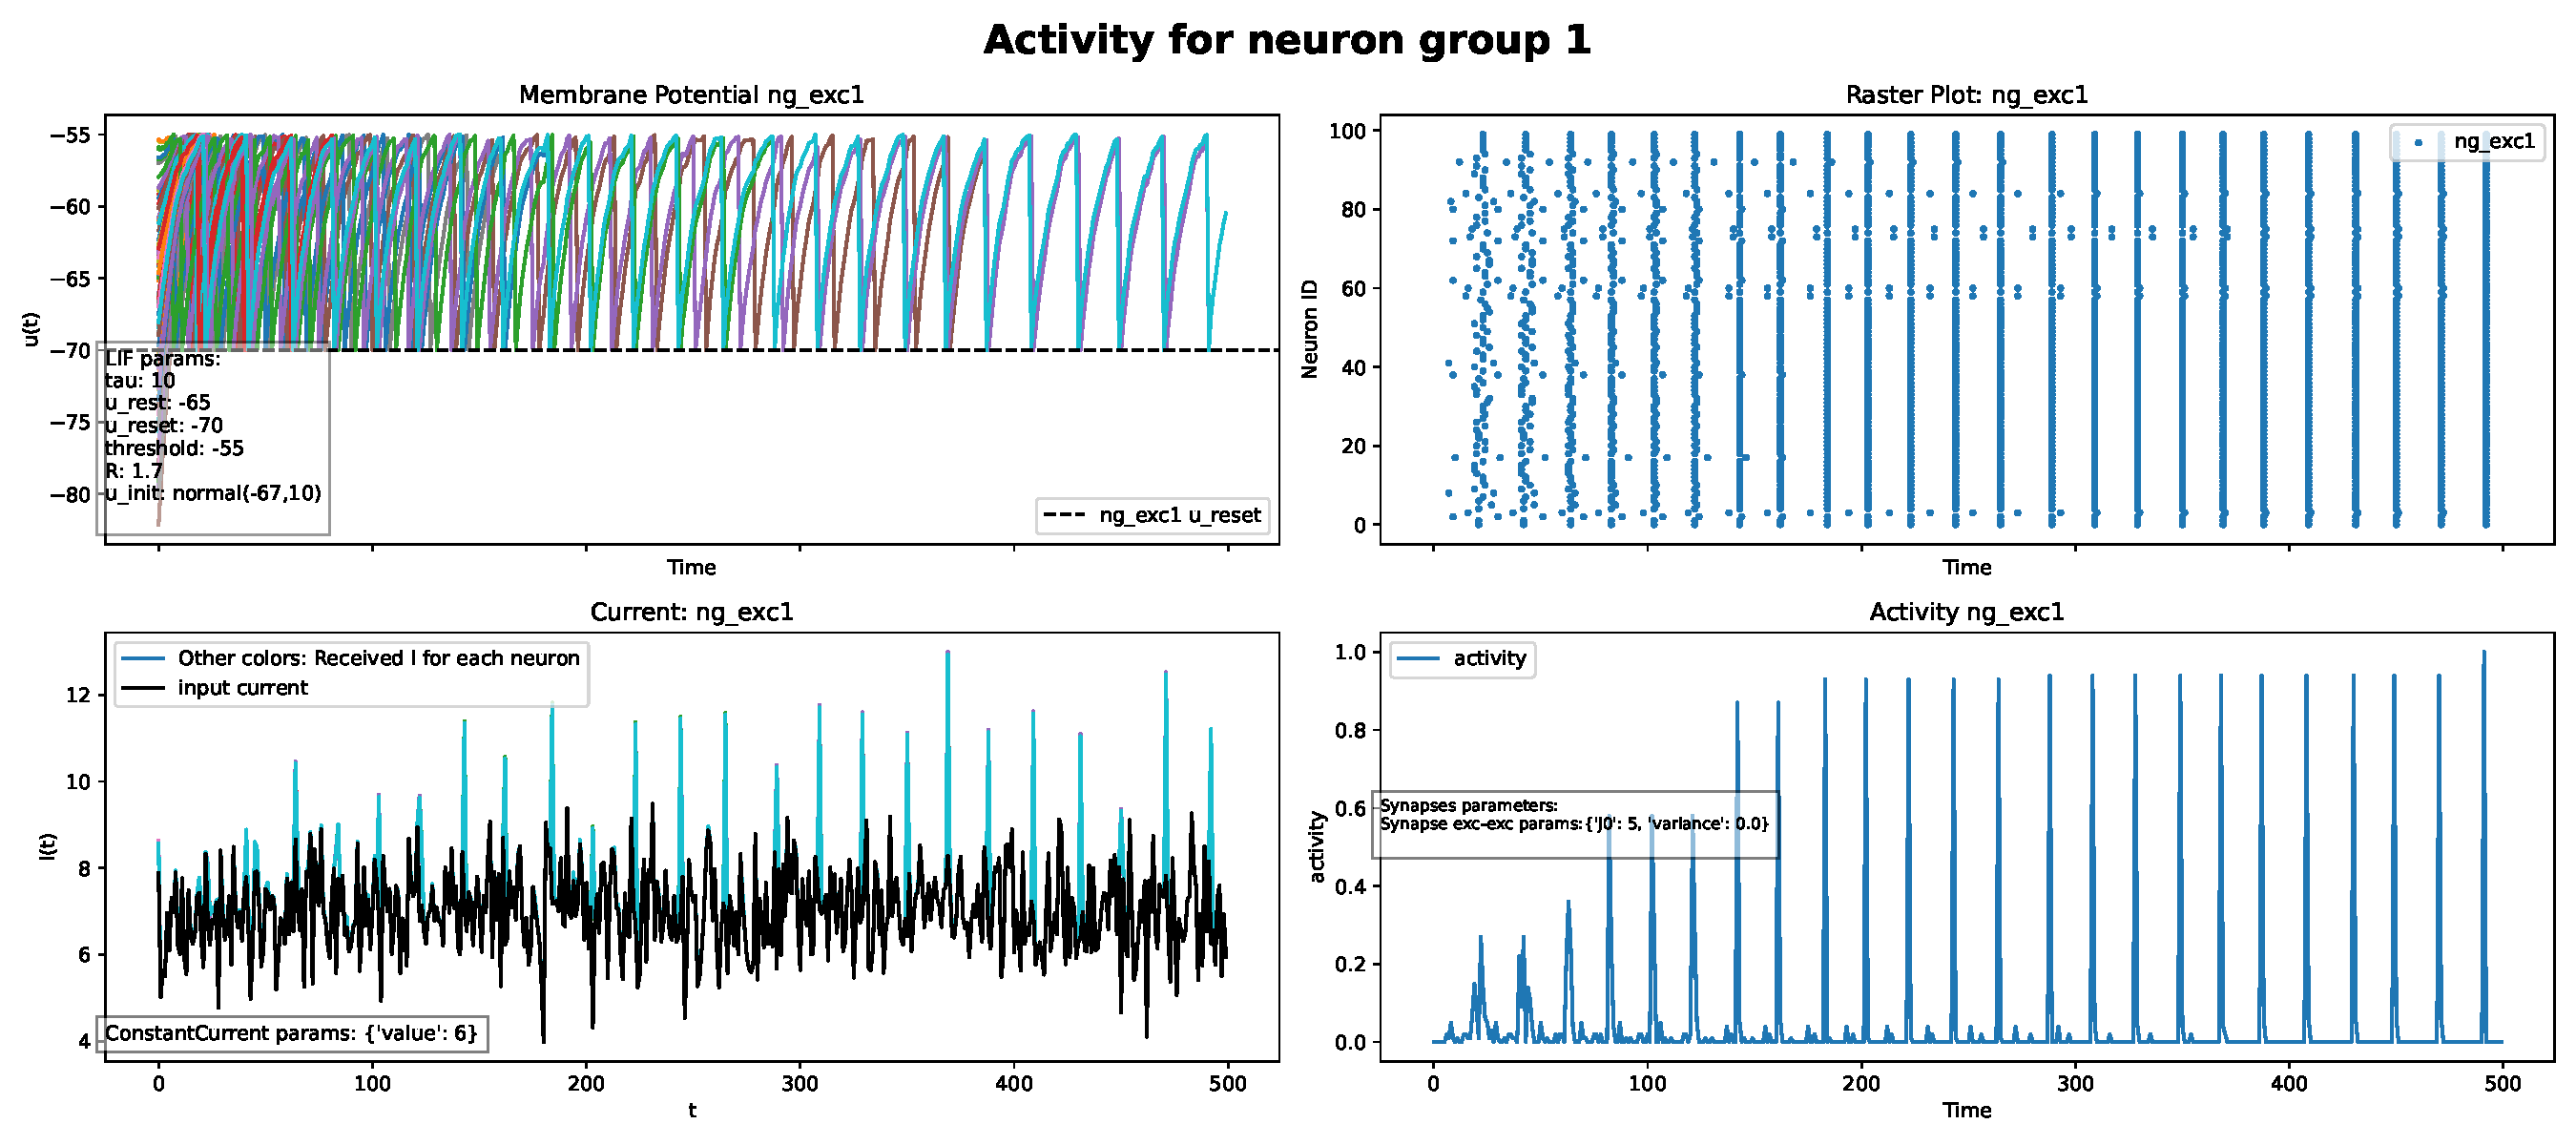
\includegraphics[width=0.9\textwidth]{plots/part1-Simple-ng-with-synapse-noise-curr.pdf} 
            \caption{جمعیت نورونی با سیناپس: اختلاف پتانسیل اولیه متفاوت و جریان نویز دار}
            \label{fig:part1-simple-ng-with-synapse-noise-curr}
        \end{figure}

        اکنون نوبت به آزمایش رفتار جمعیت نسبت به جریان متفاوت می رسد. در این آزمایش، رفتار جمعیت را با جریان نویزی برای نورون های مختلف با دامنه نوسان 0.6 بررسی میکنیم. همانطور که در شکل
        \ref{fig:part1-simple-ng-with-synapse-diff-curr}
        مشاهده می شود، داشتن جریان های متفاوت سبب می شود که زمان ضربه زدن نورون ها پارکندگی بیشتر نسبت به قبل داشته باشد ولی برخلاف جمعیت بدون سیناپس که این پراکندگی کاهش نمی یافت، در جمعیت دارای سیناپس مشاهده میکنیم که پس از مدتی، پراکندگی زمان ضربه زدن نورون ها کاهش یافته و در نتیجه فعالیت جمعیت بیشتر میشود.
        \begin{figure}[!ht]
            \centering
            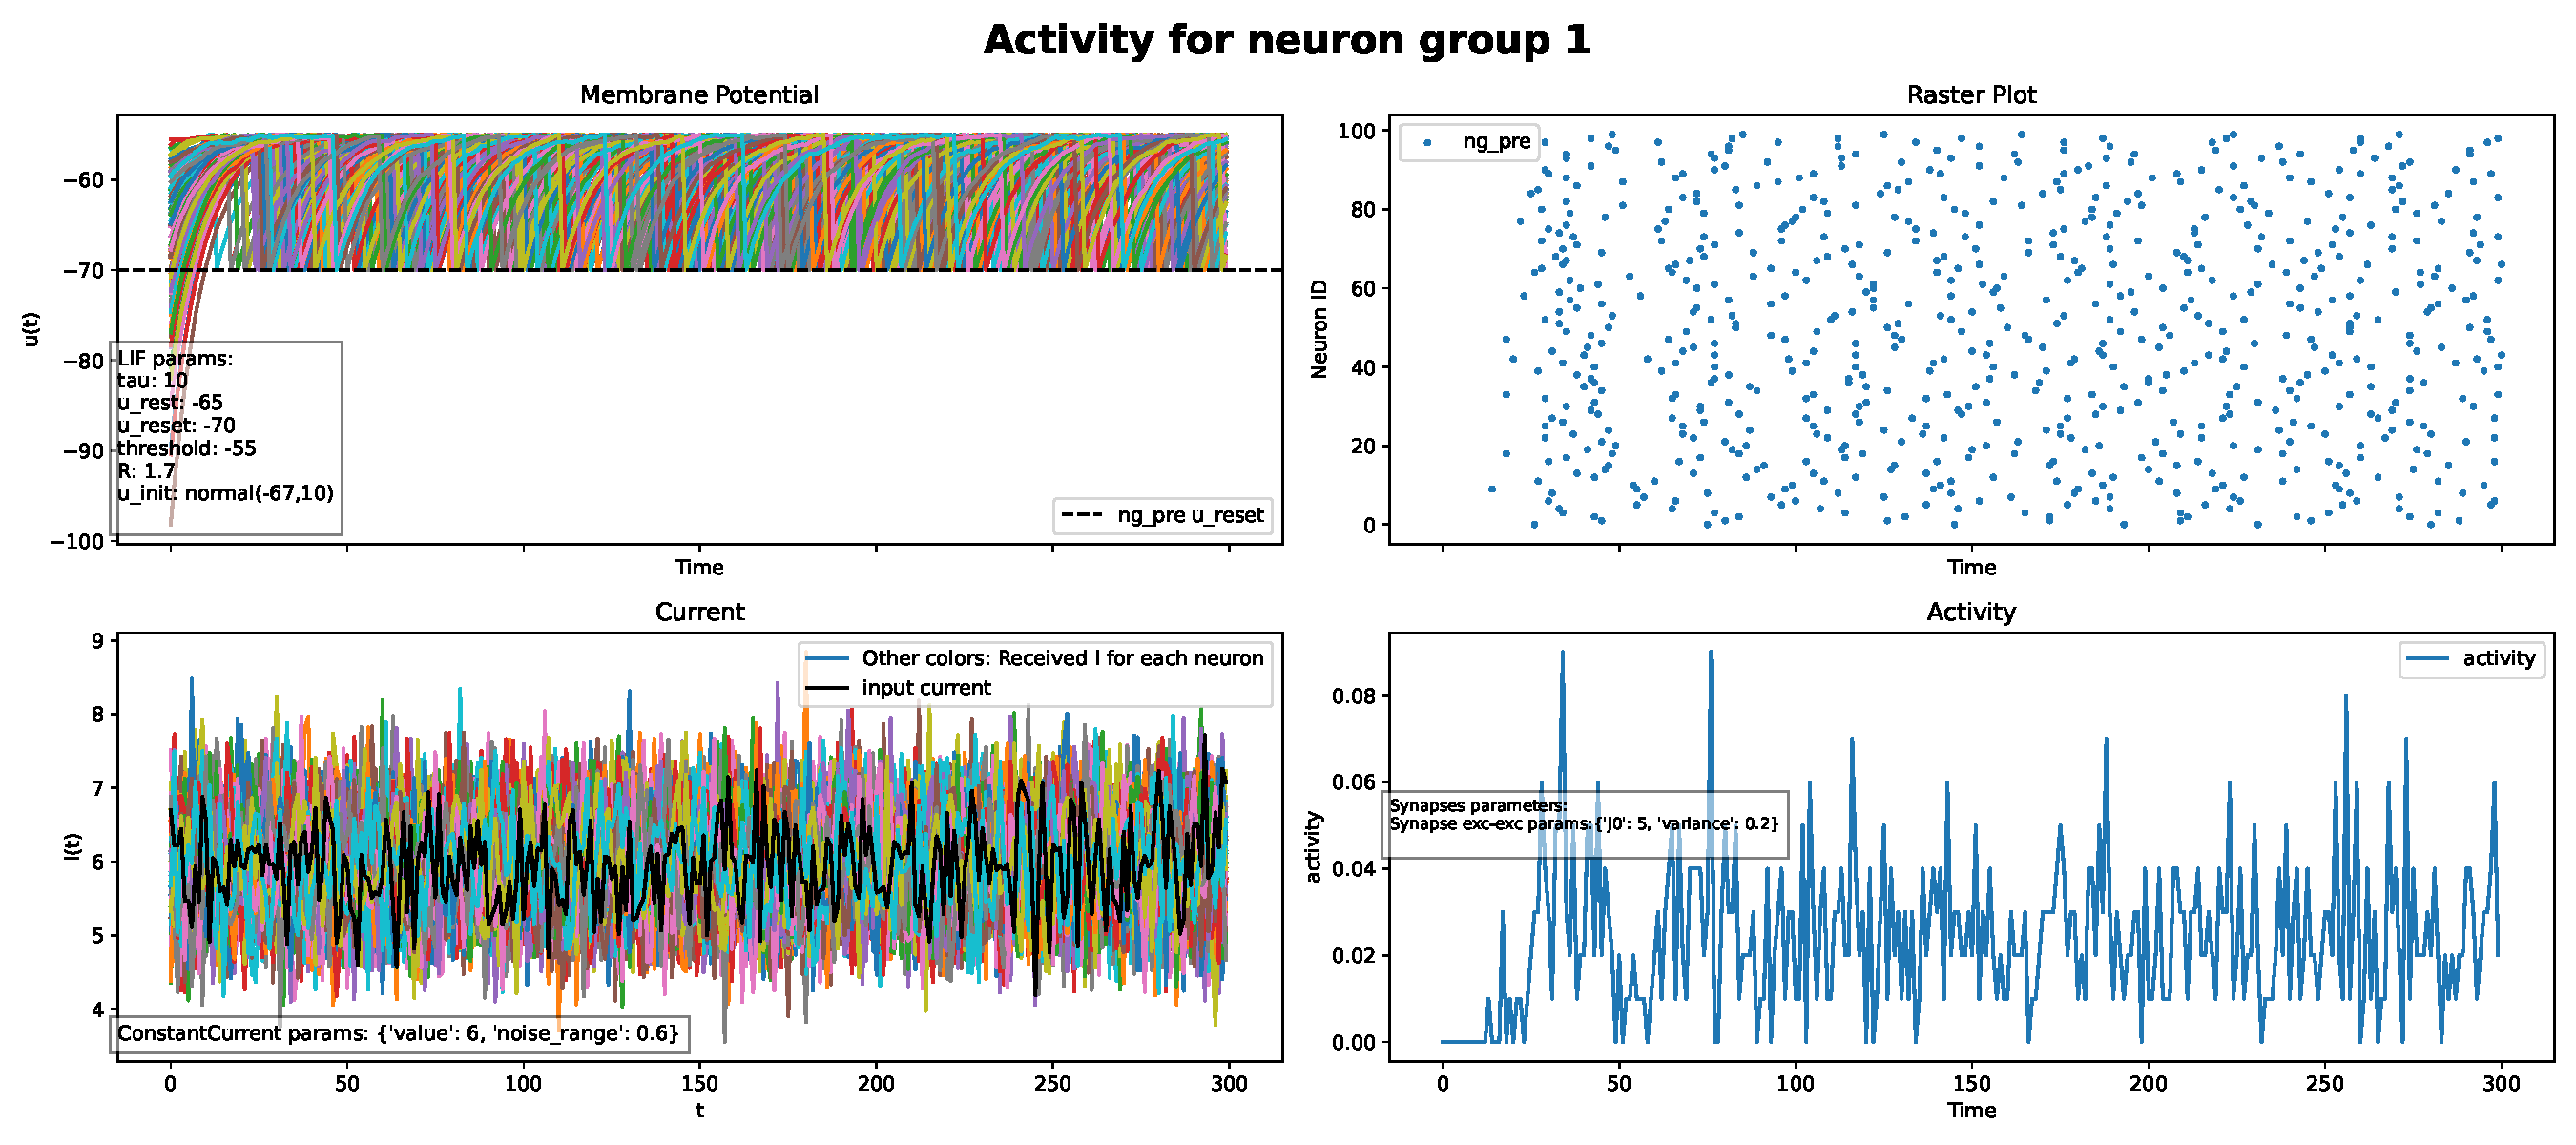
\includegraphics[width=0.9\textwidth]{plots/part1-Simple-ng-with-synapse-diff-curr.pdf} 
            \caption{جمعیت نورونی با سیناپس: اختلاف پتانسیل اولیه متفاوت و جریان نویزی غیریکسان}
            \label{fig:part1-simple-ng-with-synapse-diff-curr}
        \end{figure}

    \subsection{بررسی رفتار دو جمعیت نورونی}
        پس از بررسی رفتار یک جمعیت نورونی در حضور سیناپس، اکنون به سراغ بررسی رفتار دو جمعیت نورونی که از یکی به دیگری سیناپس وجود دارد می رویم. در این بخش تنها حالتی را در نظر میگیریم که یک جمعیت، نورون های پیش سیناپسی را تشکیل داده و جمعیت دیگر نورون های پس سیناپسی. بررسی حالت هایی با سیناپس های بیشتر را به بخش های بعدی واگذار میکنیم.

        برای اینکار، ابتدا دو جمعیت نورونی تحریکی کاملا مشابه تشکیل میدهیم که فقط از جمعیت اول به جمعیت دوم سیناپس داریم. همچنین جریان ورودی هر دو جمعیت را نیز یکسان و ثابت میگیریم. حال اگر شبیه سازی را انجام دهیم، در شکل
        \ref{fig:part1-two-ng-with-synapse}
        ملاحظه میکنیم که زمان ضربه زدن نورون های هر دو جمعیت کاملا یکسان است که این موضوع مربوط به کاملا یکسان بودن این دو جمعیت است. همچنین به دلیل اینکه در پیاده سازی سیناپس، طبق گفته حل تمرین مربوطه، نیازی نیست تا تاثیر سیناپس تا لحظات بعد نیز باقی بماند، عملا افزایش لحظه ای جریان ورودی به نورون های پس سیناپسی بی تاثیر می شود. اما اگر بتوان تاثیر جریان های موجود در سیناپس را حفظ نمود، ضربه های نورون پیش سیناپسی نیز روی نورون های پس سیناپسی تاثیر گذار خواهد بود
        (شکل \ref{fig:part1-two-ng-with-synapse-decay})
        \begin{figure}[!ht]
            \centering
            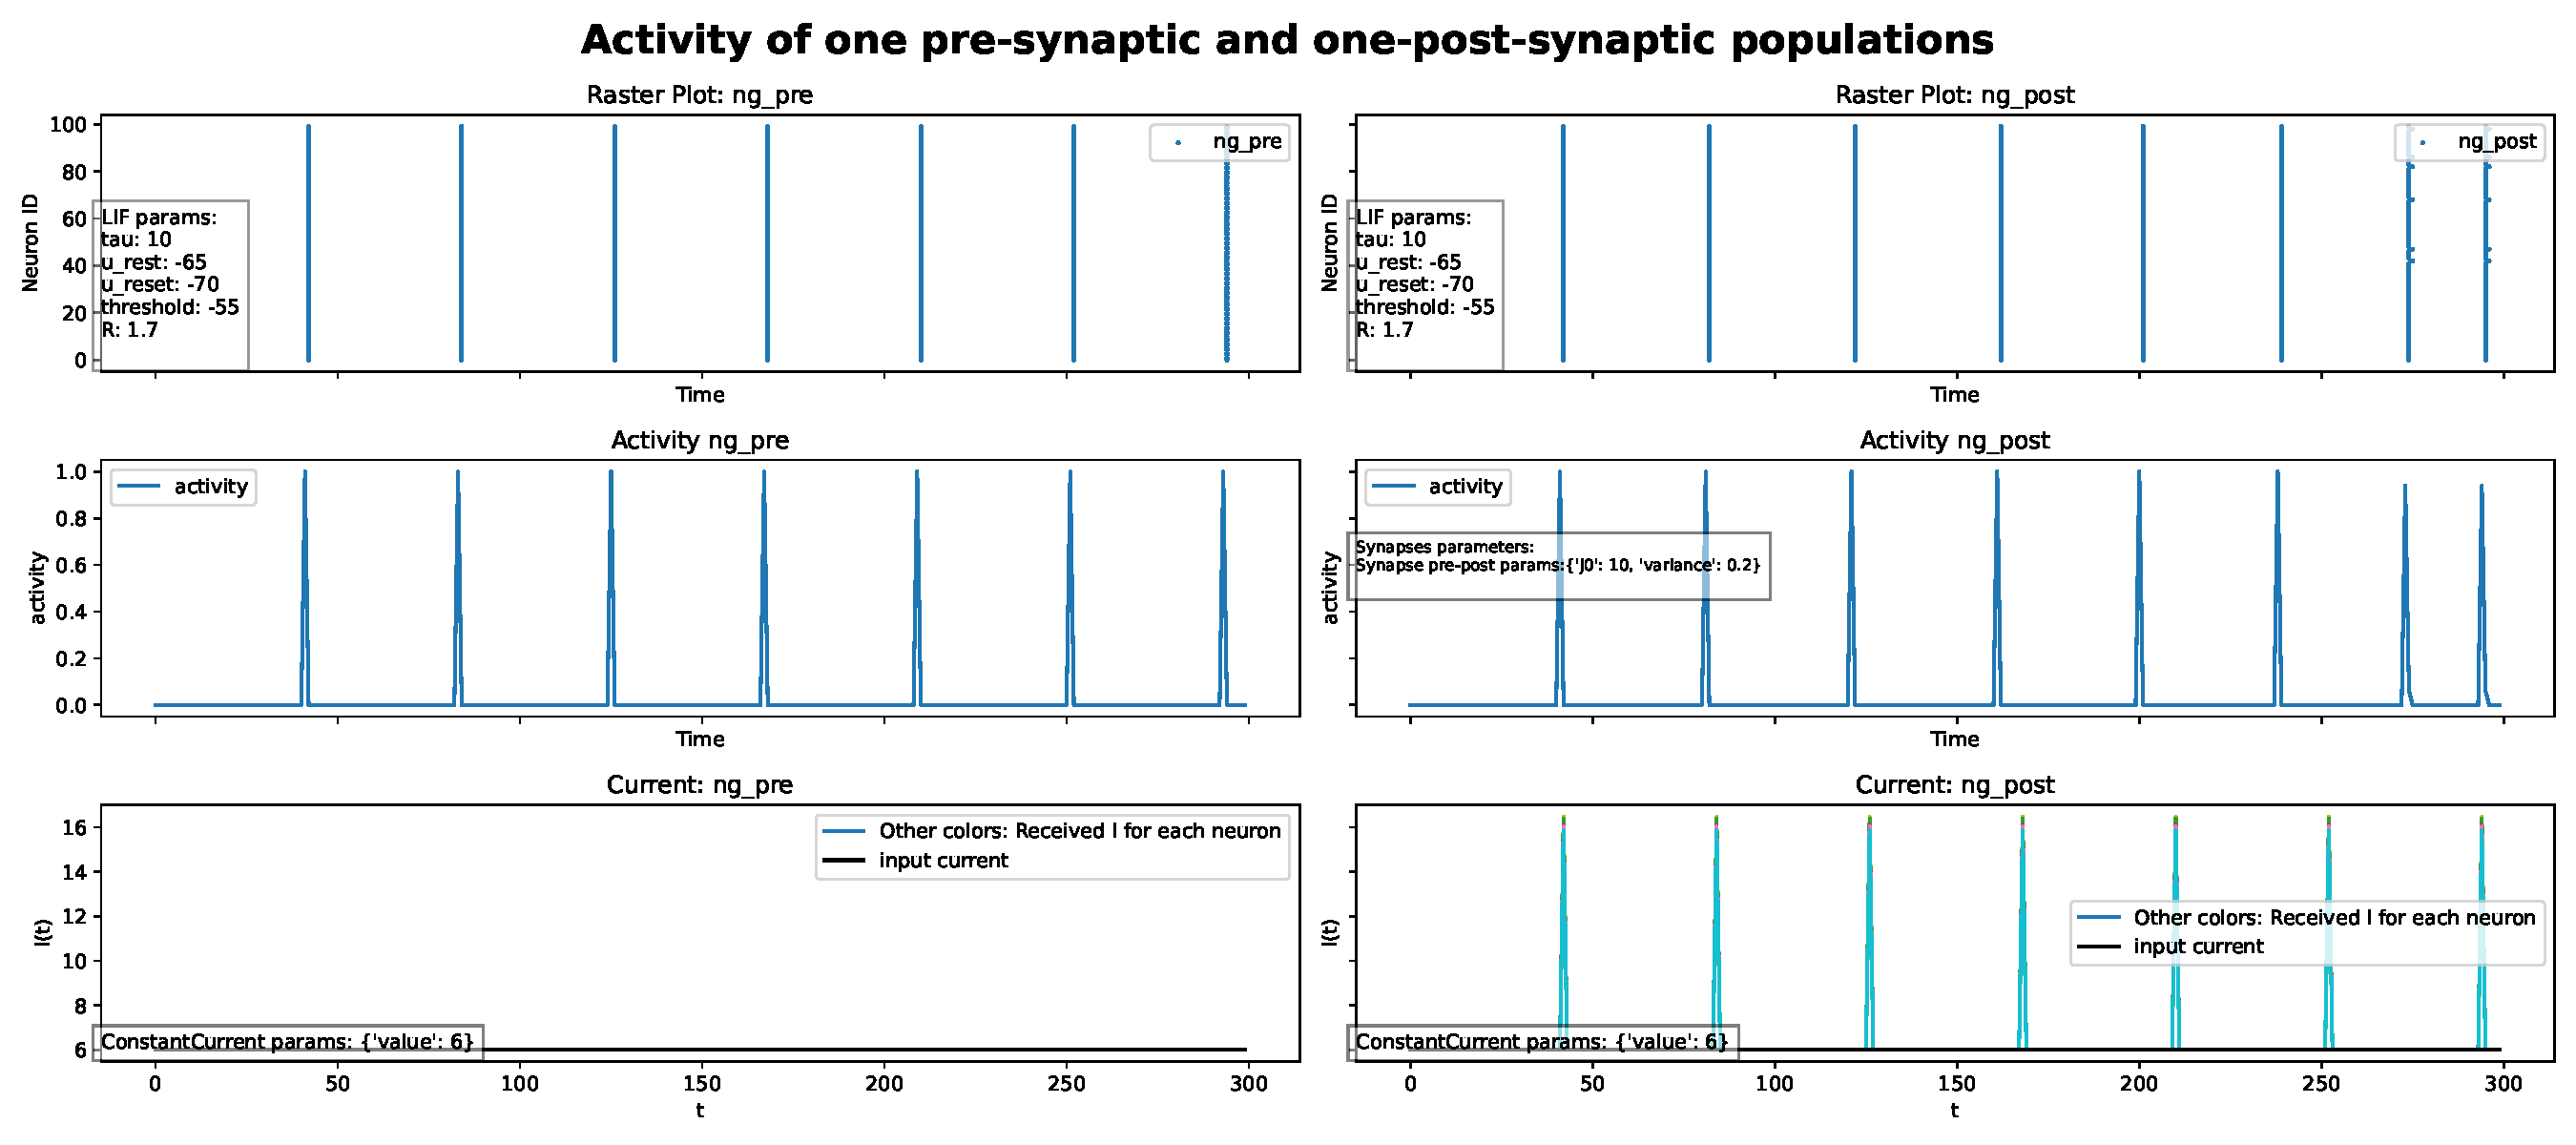
\includegraphics[width=0.9\textwidth]{plots/part1-two-ng-with-synapse.pdf} 
            \caption{جمعیت نورونی پیش سیناپسی و پس سیناپسی}
            \label{fig:part1-two-ng-with-synapse}
        \end{figure}
        \begin{figure}[!ht]
            \centering
            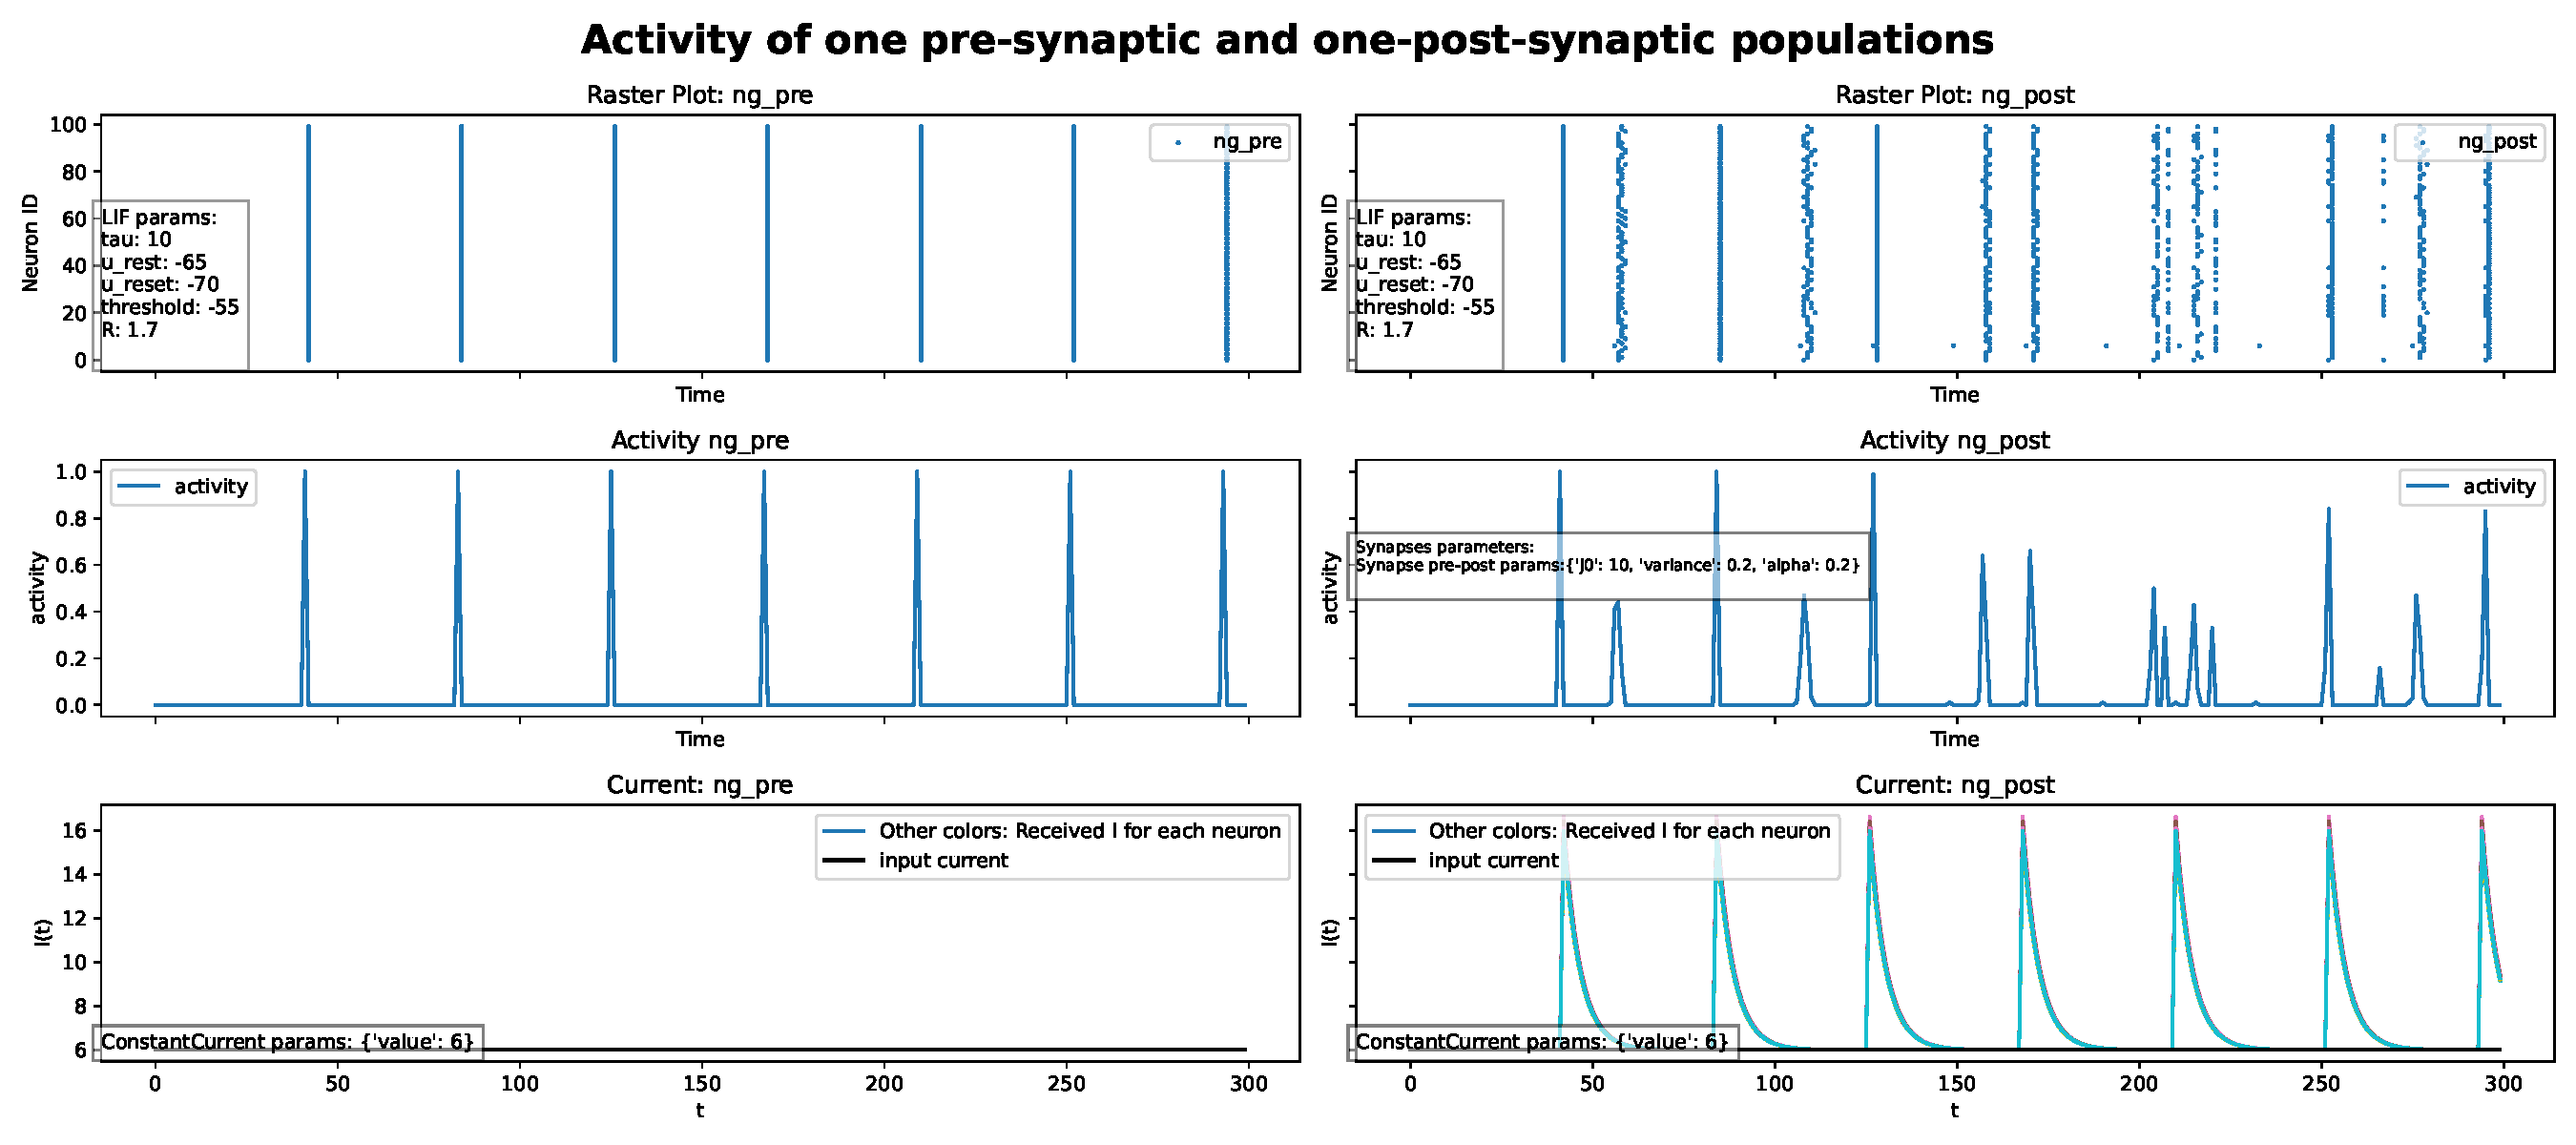
\includegraphics[width=0.9\textwidth]{plots/part1-two-ng-with-synapse-decay.pdf} 
            \caption{جمعیت نورونی پیش سیناپسی و پس سیناپسی: حفظ تاثیر جریان سیناپسی تا لحظات بعد}
            \label{fig:part1-two-ng-with-synapse-decay}
        \end{figure}
        به دلیل اینکه این نوع سیناپس هدف اصلی پروژه نمی باشد، ما بررسی های خود را بیشتر روی همان حالت گفته شده توسط دستیار آموزشی انجام می دهیم.
        
        حال اگر به نمودار 
        \ref{fig:part1-two-ng-with-synapse}
        اختلاف پتانسیل اولیه متفاوت بیفزاییم، طبق شکل 
        \ref{fig:part1-two-ng-with-synapse-u-init}
        ملاحظه میکنیم که فواصل زمانی ضربه ها در جمعیت دوم نزدیک تر بوده و فعالیت آن نسبت به جمعیت اول بیشتر است. این به این دلیل است که در جمعیت دوم، علاوه بر جریان ورودی، جریان سیناپسی که از جمعیت اول گرفته می شود نیز وجود دارد.
        \begin{figure}[!ht]
            \centering
            \includegraphics[width=0.9\textwidth]{plots/part1-two-ng-with-synapse-u\_init.pdf} 
            \caption{جمعیت نورونی پیش سیناپسی و پس سیناپسی: تاثیر اختلاف پتانسیل اولیه متفاوت}
            \label{fig:part1-two-ng-with-synapse-u-init}
        \end{figure}

        حال به جریان ورودی هر دو جمعیت، یک جریان یکسان نویز دار اضافه میکنیم. همانطور که در شکل
        \ref{fig:part1-two-ng-with-synapse-noise-curr}
        ملاحظه میکنیم، با اینکه نویز اضافه شده به هر دو نمودار از توزیع یکسان
        (میانگین=۰ و واریانس=۱)
        پیروی میکند، جریان دریافتی نهایی نورون های جمعیت پس سیناپسی، به طور میانگین بیشتر از جمعیت نورونی پیش سیناپسی است و در نتیجه فعالیت جمعیت آن نیز بیشتر است. این به این دلیل است که جریانی تحت تاثیر ضربه های جمعیت پیش سیناپسی به جریان جمعیت پس سیناپسی نیز اضافه می شود.
        \begin{figure}[!ht]
            \centering
            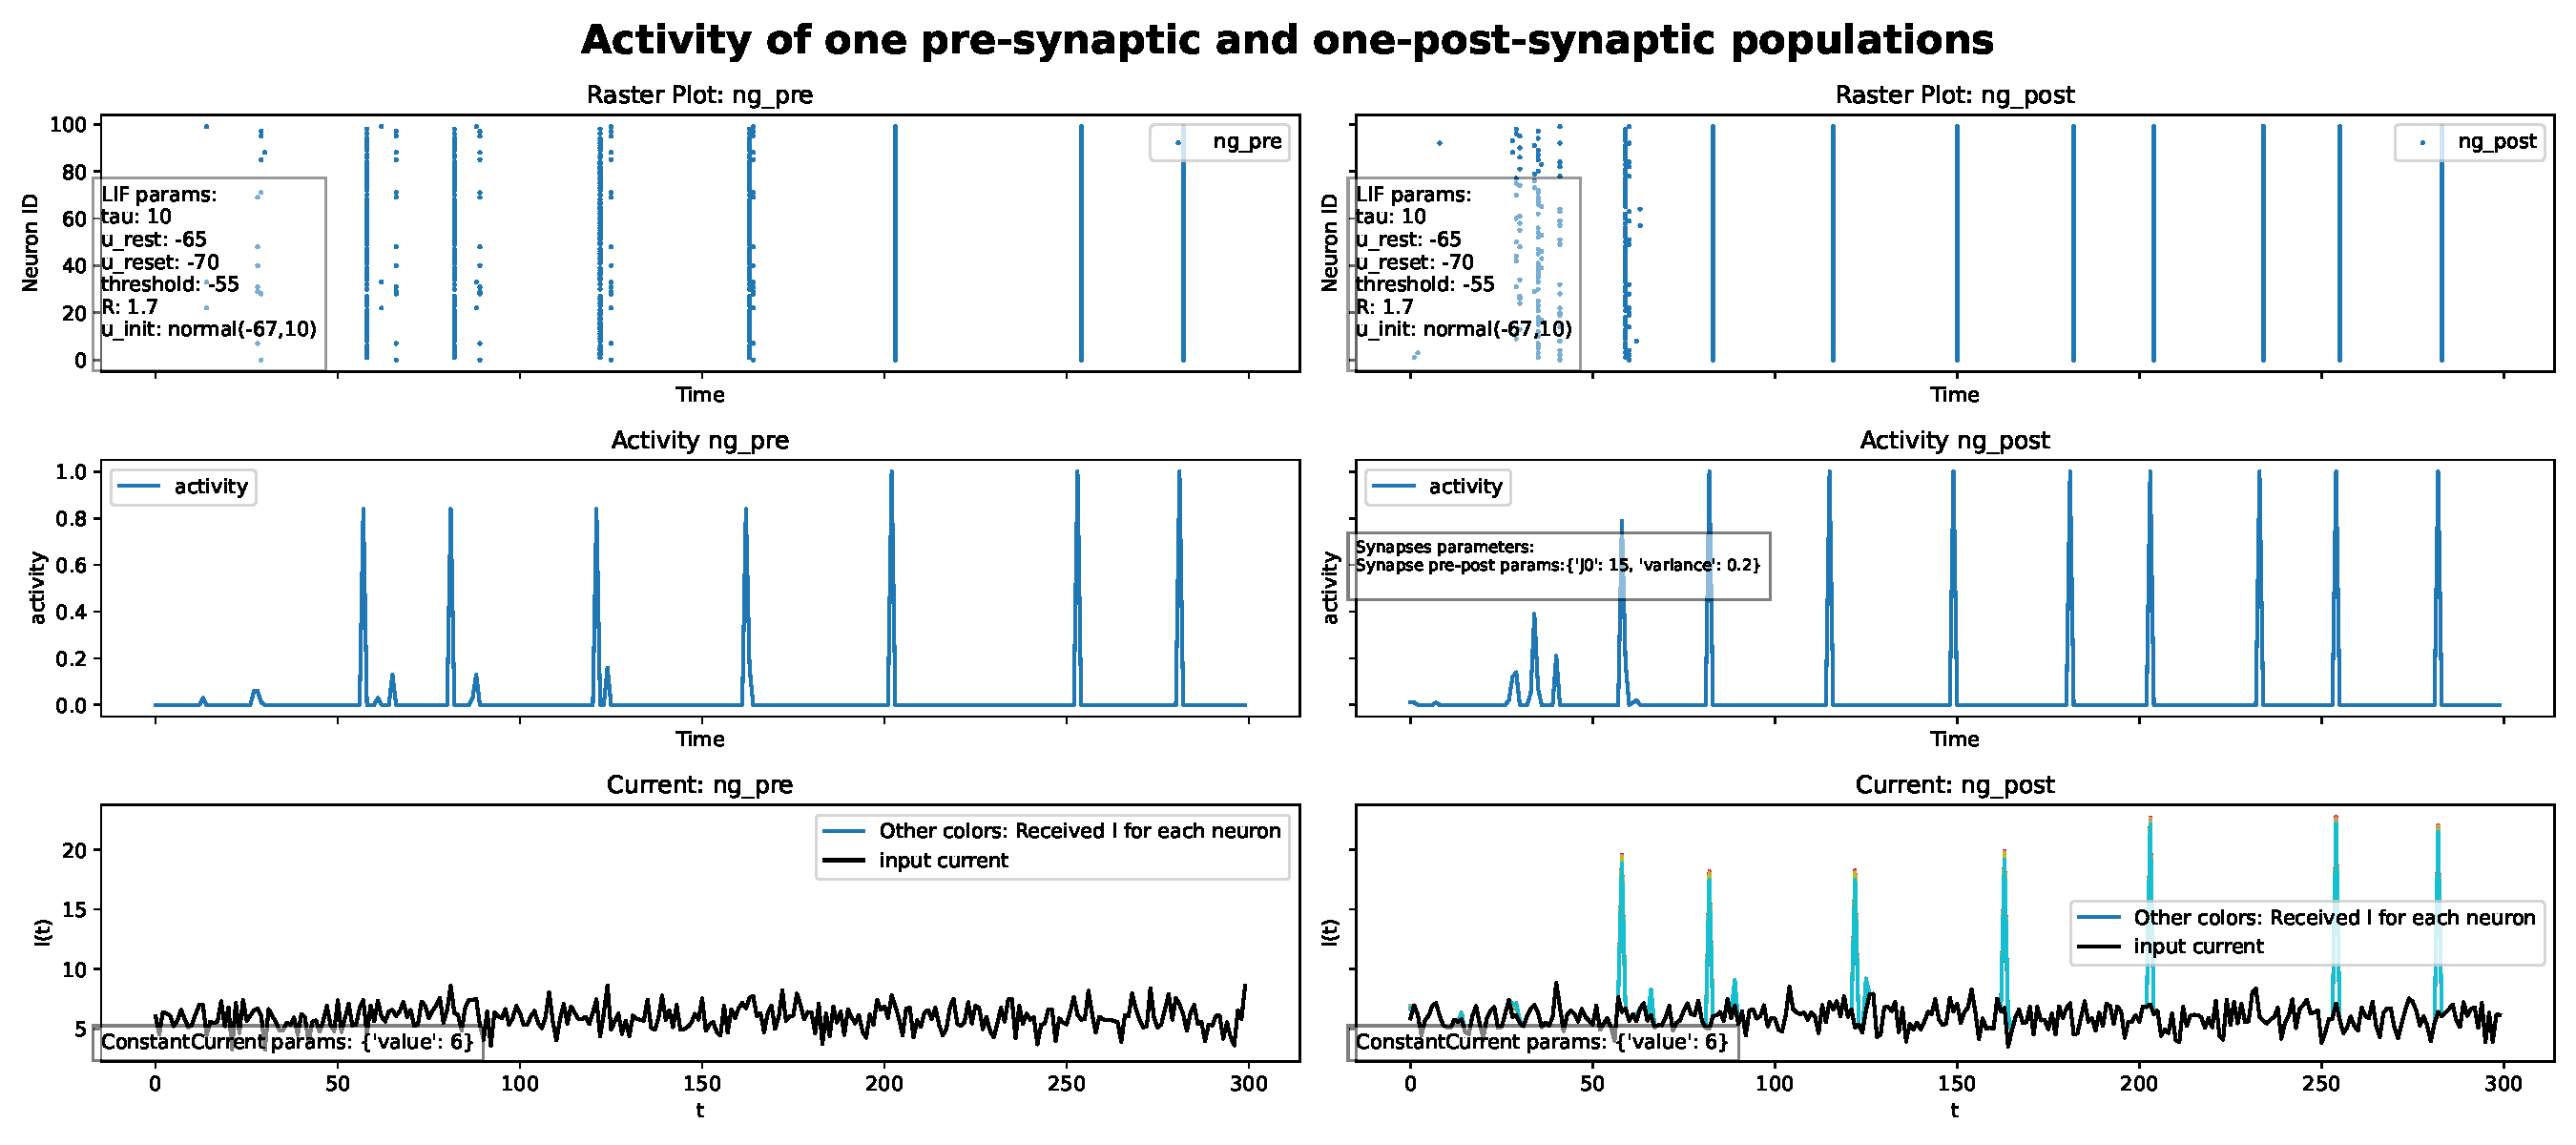
\includegraphics[width=0.9\textwidth]{plots/part1-two-ng-with-synapse-noise-curr.pdf} 
            \caption{جمعیت نورونی پیش سیناپسی و پس سیناپسی: تاثیر جریان نویزی}
            \label{fig:part1-two-ng-with-synapse-noise-curr}
        \end{figure}

        حال رفتار جمعیت را با جریان نویزی غیریکسان آزمایش میکنیم. دامنه نوسان را 
        $0.2$ 
        تنظیم میکنیم و انتظار داریم که مانند شکل های گذشته، میزان پراکندگی زمان ضربه زدن های نورون ها بیشتر شود، که از شکل 
        \ref{fig:part1-two-ng-with-synapse-diff-curr}
        نیز همین دریافت می شود.
        \begin{figure}[!ht]
            \centering
            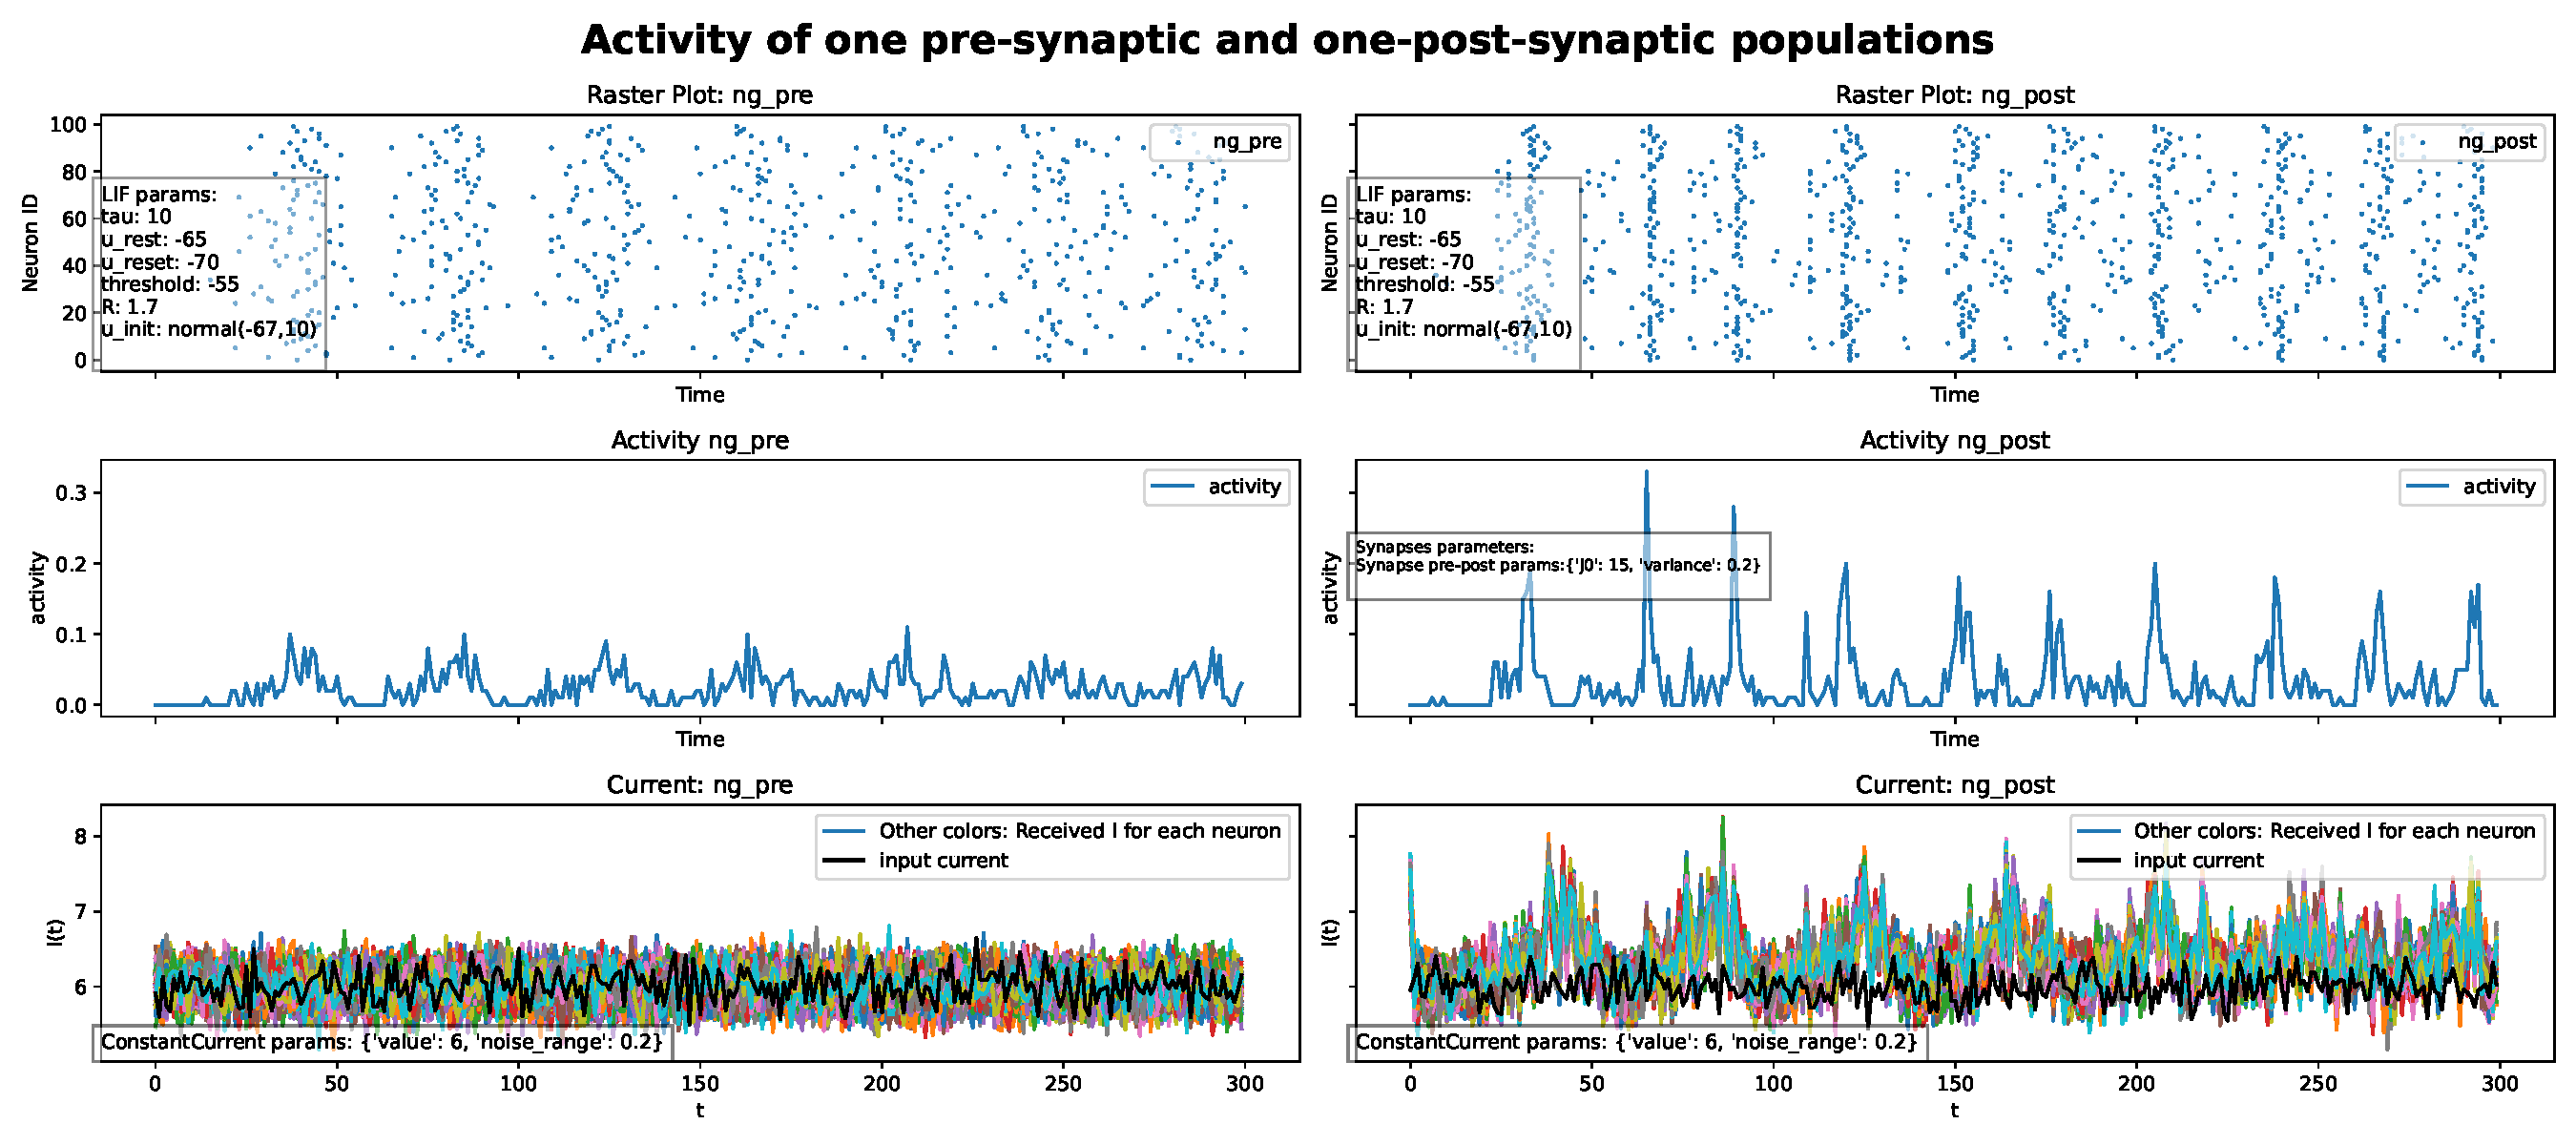
\includegraphics[width=0.9\textwidth]{plots/part1-two-ng-with-synapse-diff-curr.pdf} 
            \caption{جمعیت نورونی پیش سیناپسی و پس سیناپسی: تاثیر جریان نویزی غیریکسان}
            \label{fig:part1-two-ng-with-synapse-diff-curr}
        \end{figure}

        اگر دامنه نوسان جریان را تا 
        $0.5$ 
        بیشتر افزایش دهیم، هرچند پراکندگی زمان ضربه زدن هر دو جمعیت بیشتر می شود، ولی هنوز بیشتر بودن فعالیت جمعیت نورونی دوم مشهود است.
        (شکل \ref{fig:part1-two-ng-with-synapse-high-diff-curr})
        \begin{figure}[!ht]
            \centering
            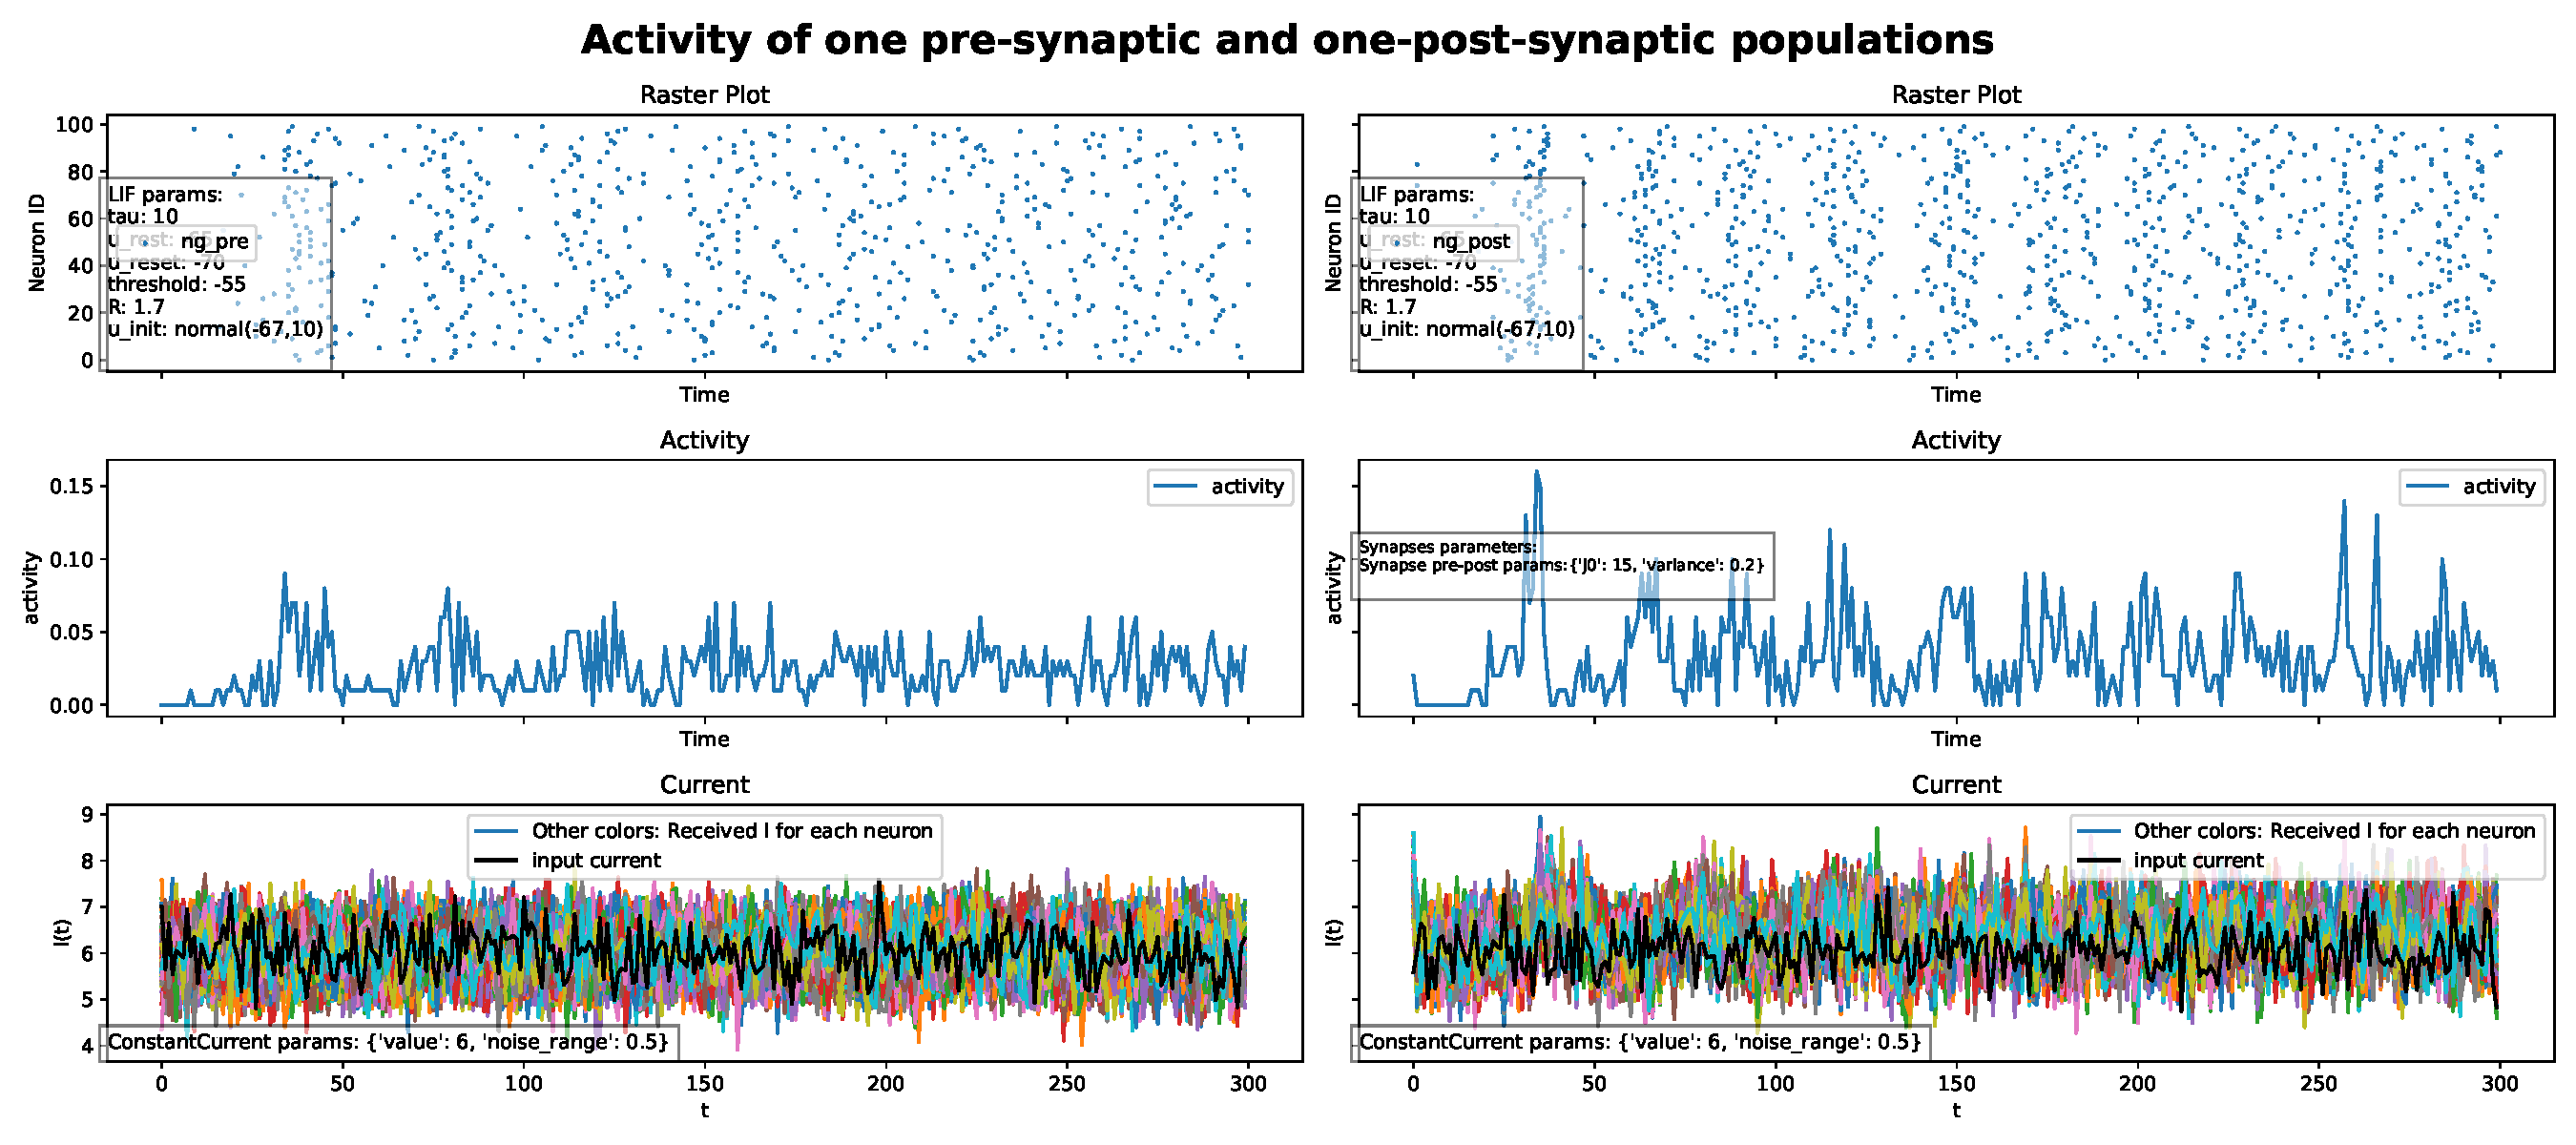
\includegraphics[width=0.9\textwidth]{plots/part1-two-ng-with-synapse-high-diff-curr.pdf} 
            \caption{جمعیت نورونی پیش سیناپسی و پس سیناپسی: تاثیر جریان نویزی غیریکسان}
            \label{fig:part1-two-ng-with-synapse-high-diff-curr}
        \end{figure}
 
        به عنوان آخرین نمودار این بخش و مقدمه ای بر بخش بعدی، افزایش مقدار 
        $j_0$ 
        را بررسی میکنیم. همانطور که از شکل 
        \ref{fig:part1-two-ng-with-synapse-high-diff-curr-high-j}
        بر می آید، افزایش 
        $j_0$ 
        منجر به افزایش وزن ها و در نتیجه افزایش جریان سیناپسی ورودی به جمعیت نورونی پس سیناپسی شده و فعالیت آن را بیشتر می کند.
        \begin{figure}[!ht]
            \centering
            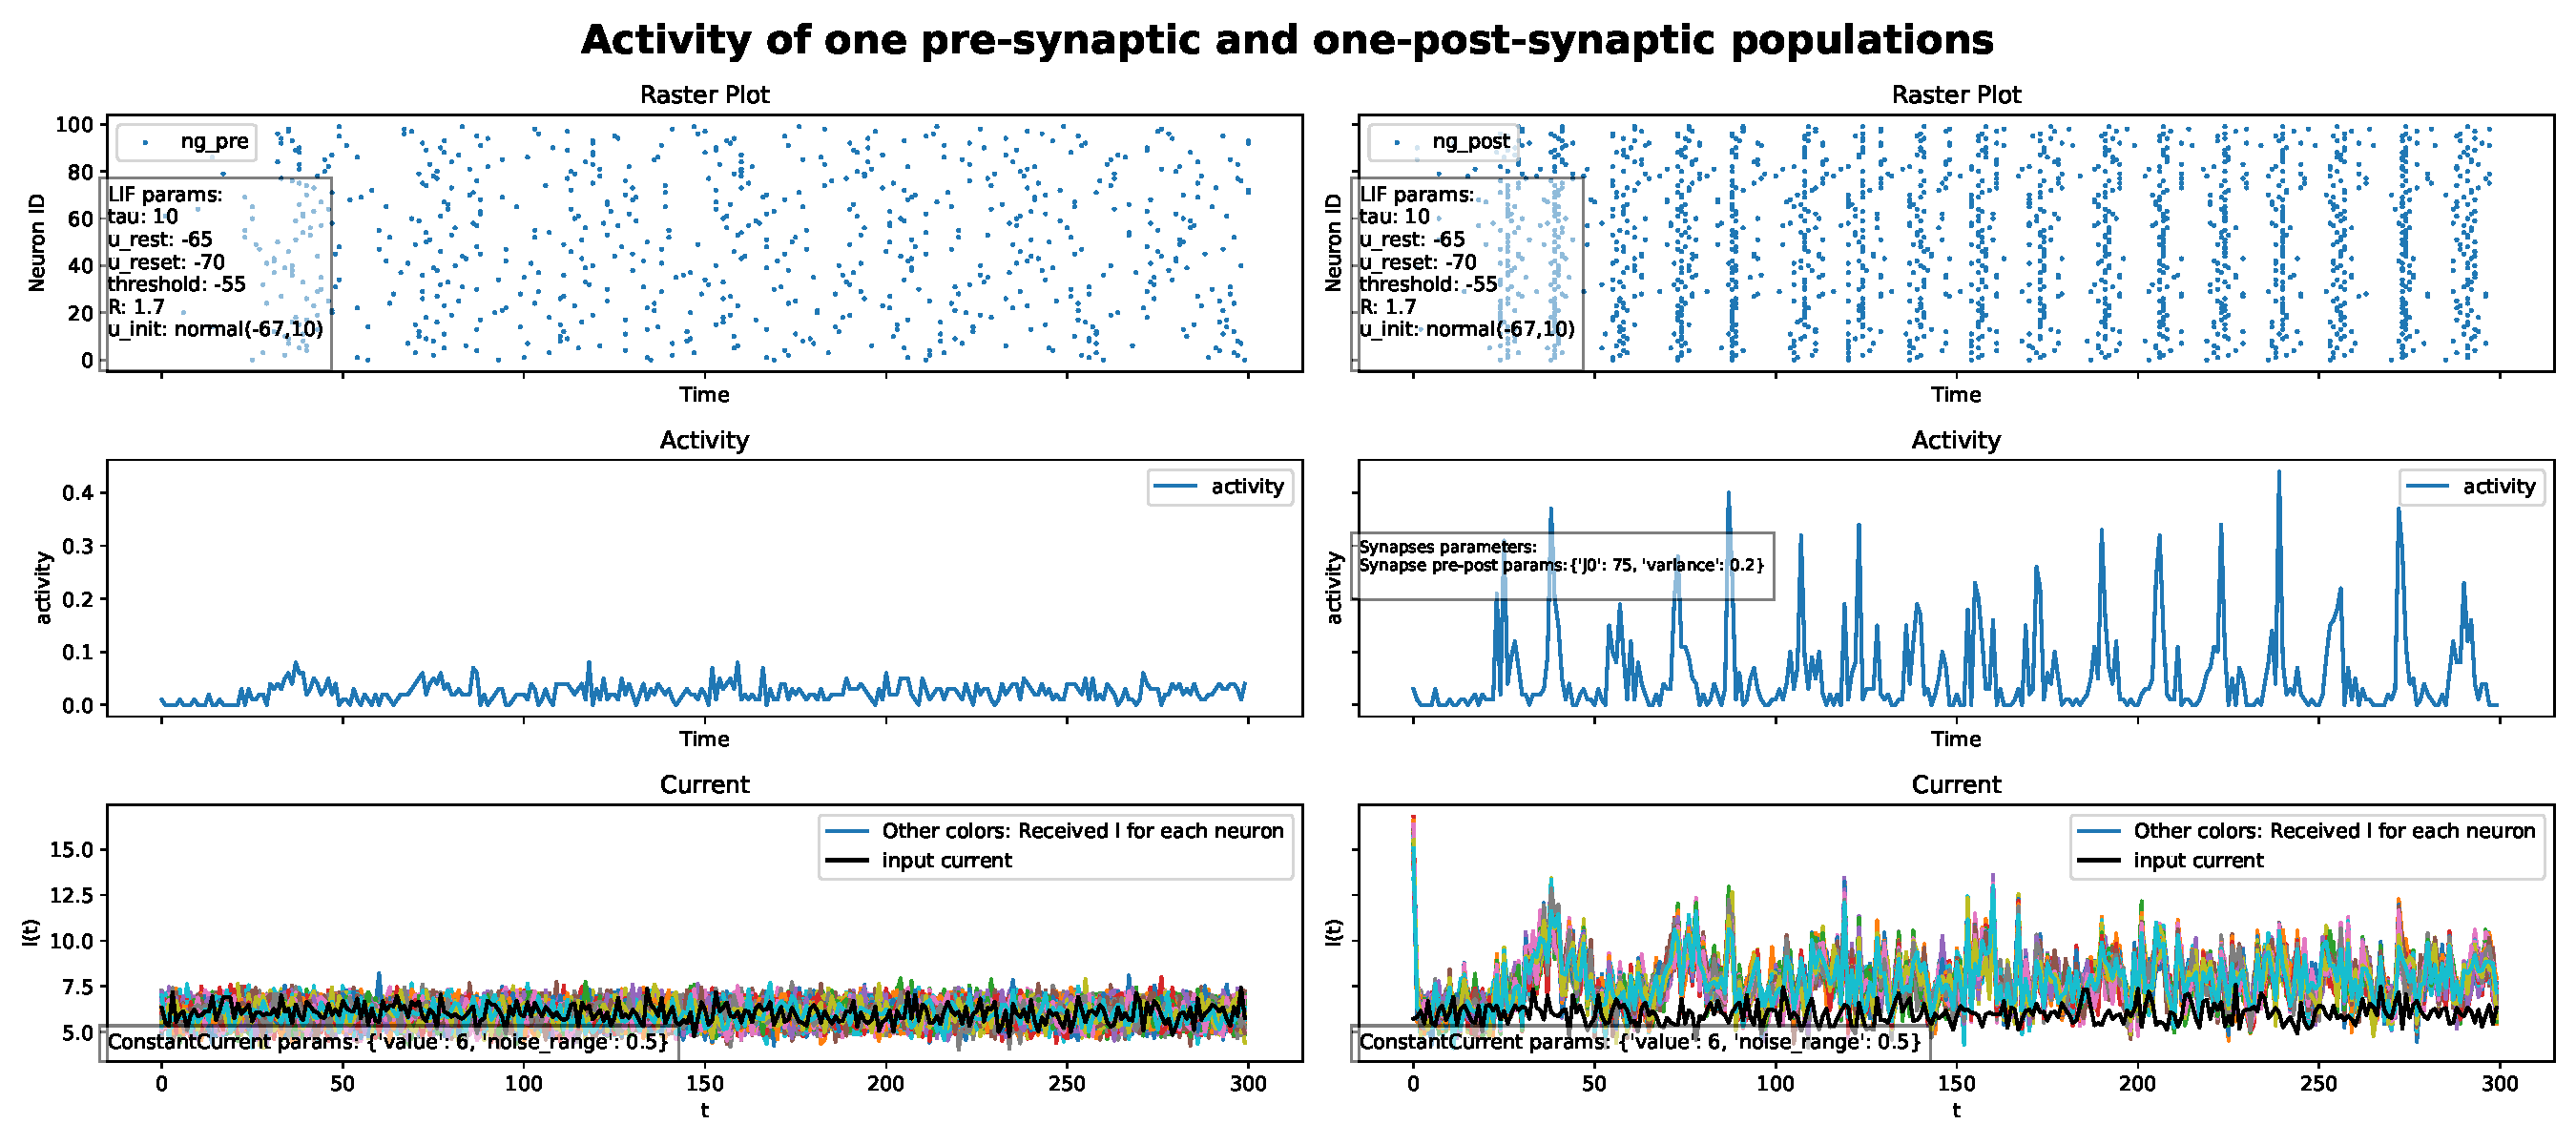
\includegraphics[width=0.9\textwidth]{plots/part1-two-ng-with-synapse-high-diff-curr-high-j.pdf} 
            \caption{جمعیت نورونی پیش سیناپسی و پس سیناپسی: تاثیر جریان نویزی غیریکسان}
            \label{fig:part1-two-ng-with-synapse-high-diff-curr-high-j}
        \end{figure}

